%%%%%%%%%%%%%%%%%%%%%%%%%%%%%%%%%%%%%%%%%%%%%%%%%%%%%%%%%%%%%%%%%%%%%%
% 
% Epistasis: Brisbane Statistical Genetics Forum 
% 
%%%%%%%%%%%%%%%%%%%%%%%%%%%%%%%%%%%%%%%%%%%%%%%%%%%%%%%%%%%%%%%%%%%%%%
%
%   Author: Joseph Powell; joseph.powell@uq.edu.au
%
%%%%%%%%%%%%%%%%%%%%%%%%%%%%%%%%%%%%%%%%%%%%%%%%%%%%%%%%%%%%%%%%%%%%%%

\documentclass{beamer}
\usepackage{beamerthemeshadow}
\usepackage[latin1]{inputenc}
\usepackage{comment}
\usetheme{Frankfurt}
%\usefonttheme{serif} 

%\setbeamercolor{structure}{rgb}{}
\usecolortheme[RGB={0,160,176}]{structure}

\usepackage[absolute,overlay]{textpos} 
\usepackage{booktabs}
\usepackage{color}
\usepackage{threeparttable}
\usepackage{multirow}
\usepackage[normalem]{ulem}

\begin{document}

\title[Epistasis influencing transcription in humans]{Detection and replication of epistasis influencing transcription in humans}
\author{Joseph Powell and Gibran Hemani}
\institute{The University of Queensland Diamantina Institute \\
\vspace{.2cm}
and \\
\vspace{.2cm}
Queensland Brain Institute}
\date{11th Oct 2013}

\begin{frame}
\titlepage
\end{frame}

%%%%%%%%%%%%%%%%%%%%%%%%%%%%%%%%%%%%%%%%%%%%%%%%%%%%%%%%
%%%%%%%%%%%%%%%%%%%%%%%%%%%%%%%%%%%%%%%%%%%%%%%%%%%%%%%%

\section{Introduction}
\subsection{}
\begin{frame}{What is epistasis?}
\begin{definition}
{The effect on the phenotype caused by locus A depends on the genotype at locus B....}
\end{definition}
\vspace{0.5cm}
Epistasis has been reported in model organisms through artificial gene knockouts, artificial line crosses and hybridisation. \\
\vspace{0.5cm}
Our aim was to systematically search for instances of epistasis amongst common variants for genetic variation that has arisen in natural populations.\end{frame}



\begin{frame}{Gene expression}
\begin{columns}[c]
\column{.5\textwidth} 
\begin{itemize}
\item Transcription measured for thousands of genes
\vspace{0.3cm}
\item Typically heritable 
\vspace{0.3cm}
\item Loci (eQTLs) commonly have very large effect sizes
\vspace{0.3cm}
\item Good candidates to search for epistasis
\end{itemize}
\column{.5\textwidth}
\begin{center}
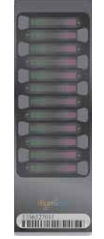
\includegraphics[width=2.0cm]{images/ht12.png}
\end{center}
\end{columns}
\end{frame}



%%%%%%%%%%%%%%%%%%%%%%%%%%%%%%%%%%%%%%%%%%%%%%%%%%%%%%%%
%%%%%%%%%%%%%%%%%%%%%%%%%%%%%%%%%%%%%%%%%%%%%%%%%%%%%%%%


\section{Methods}
\subsection{}
\begin{frame}
\begin{center}
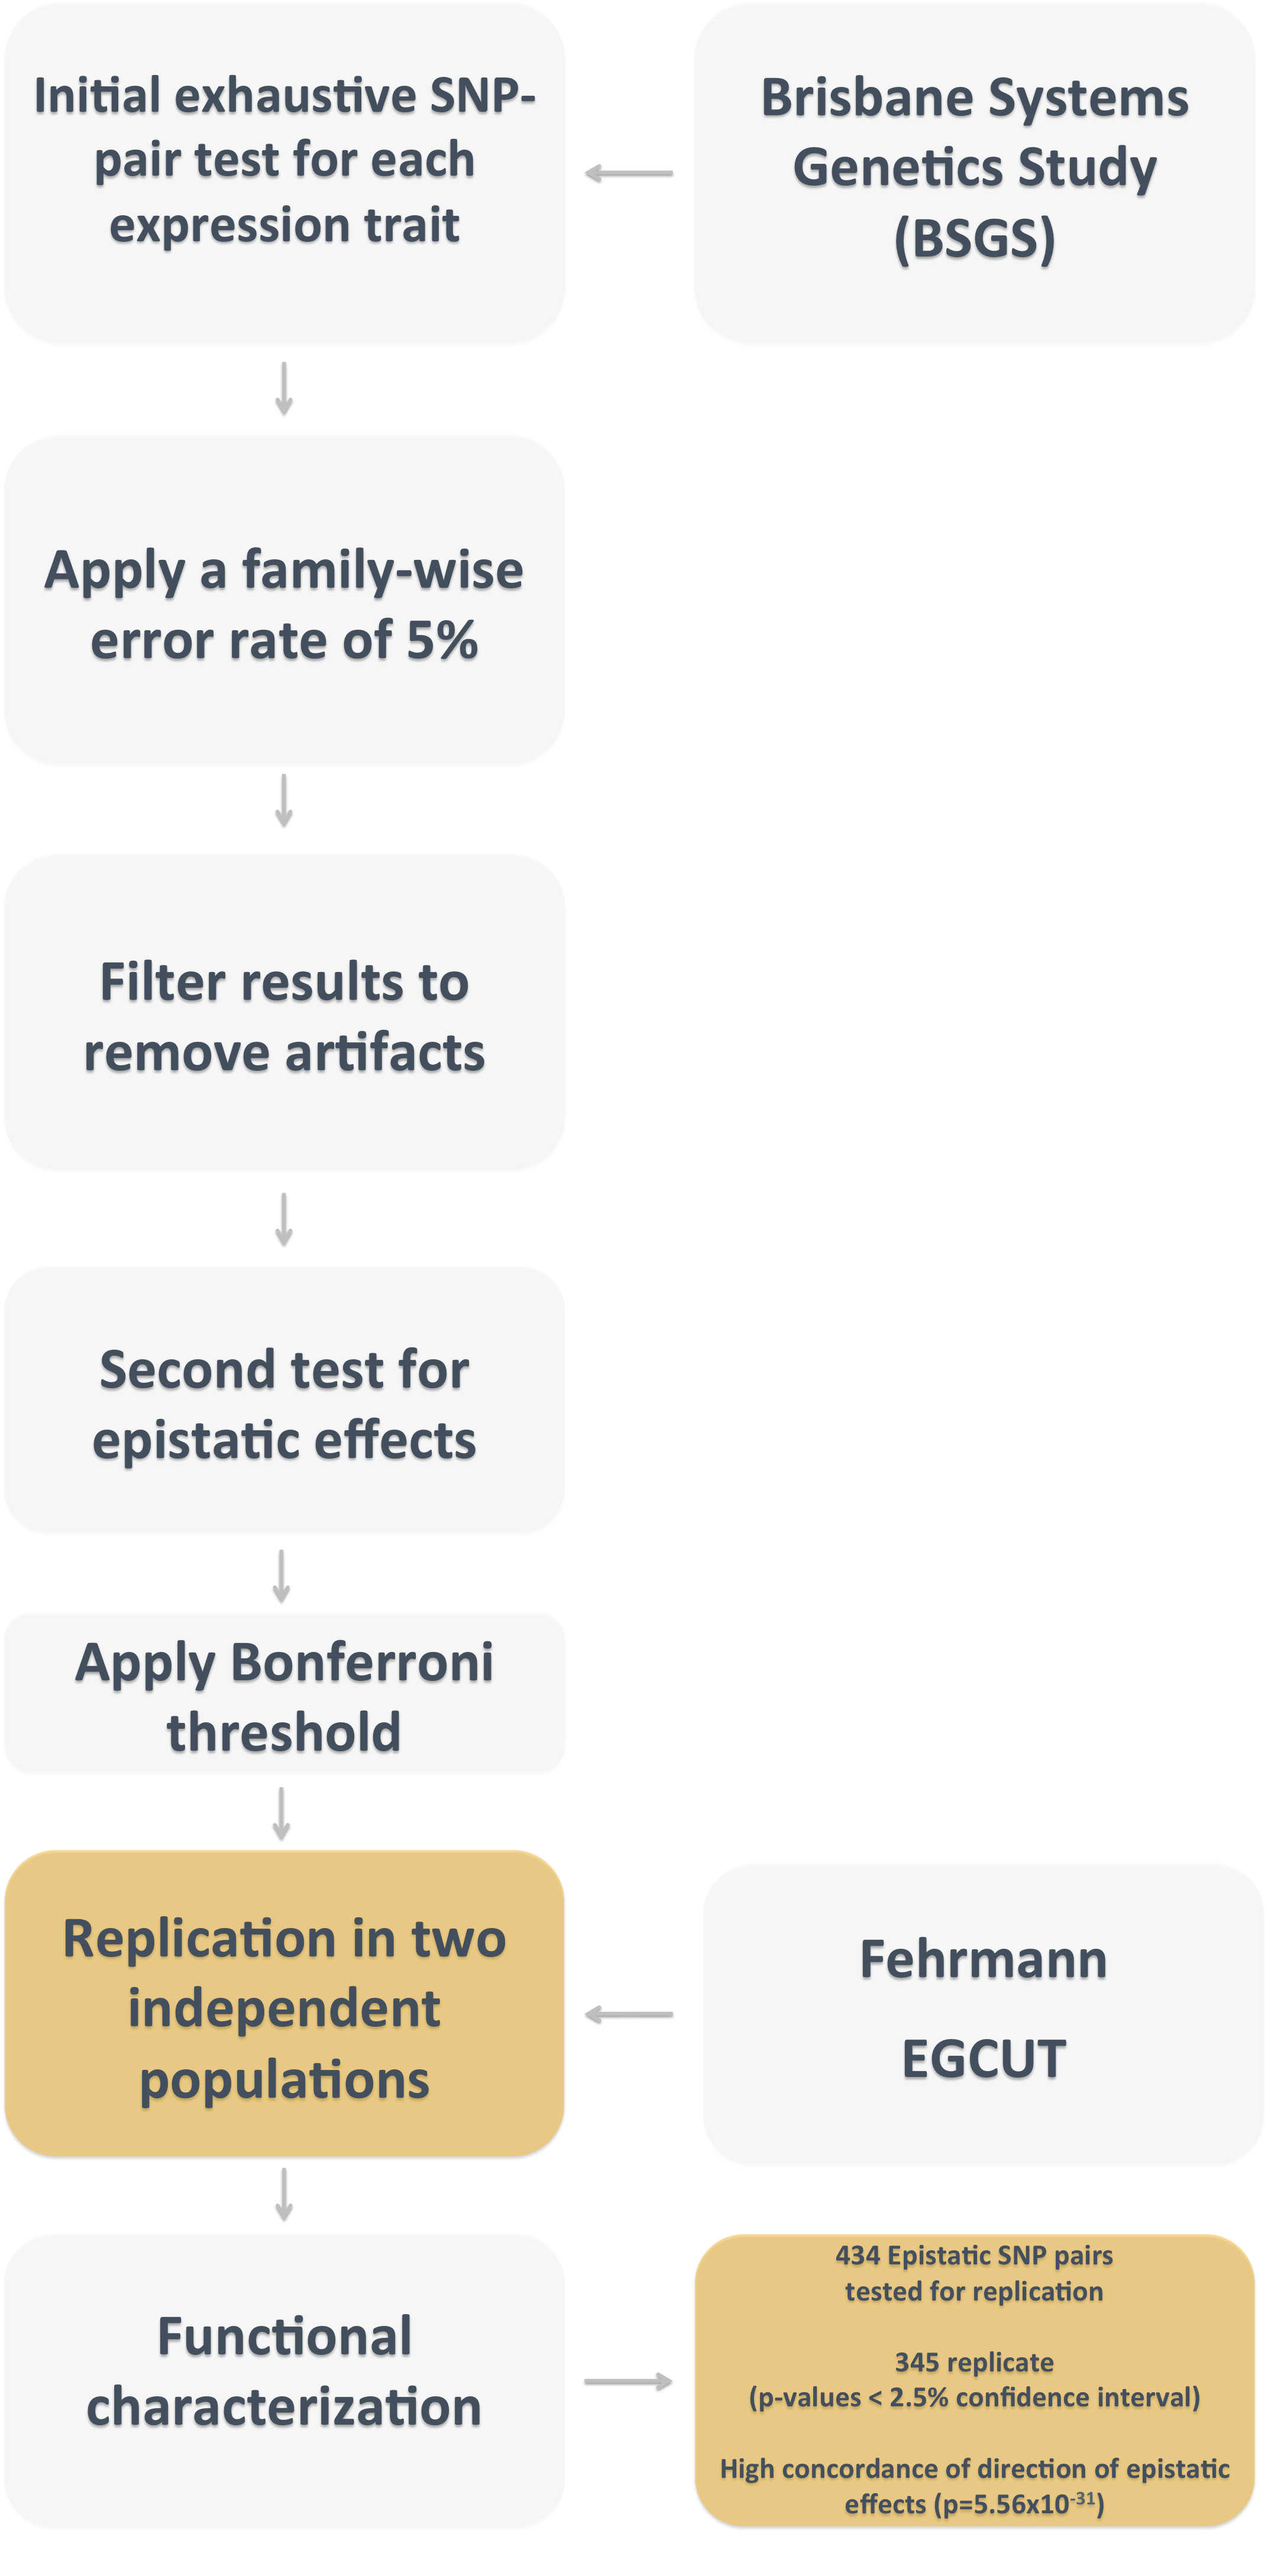
\includegraphics[height=7cm]{images/methods1.png} \\
\end{center}
\end{frame}

\begin{frame}
\begin{center}
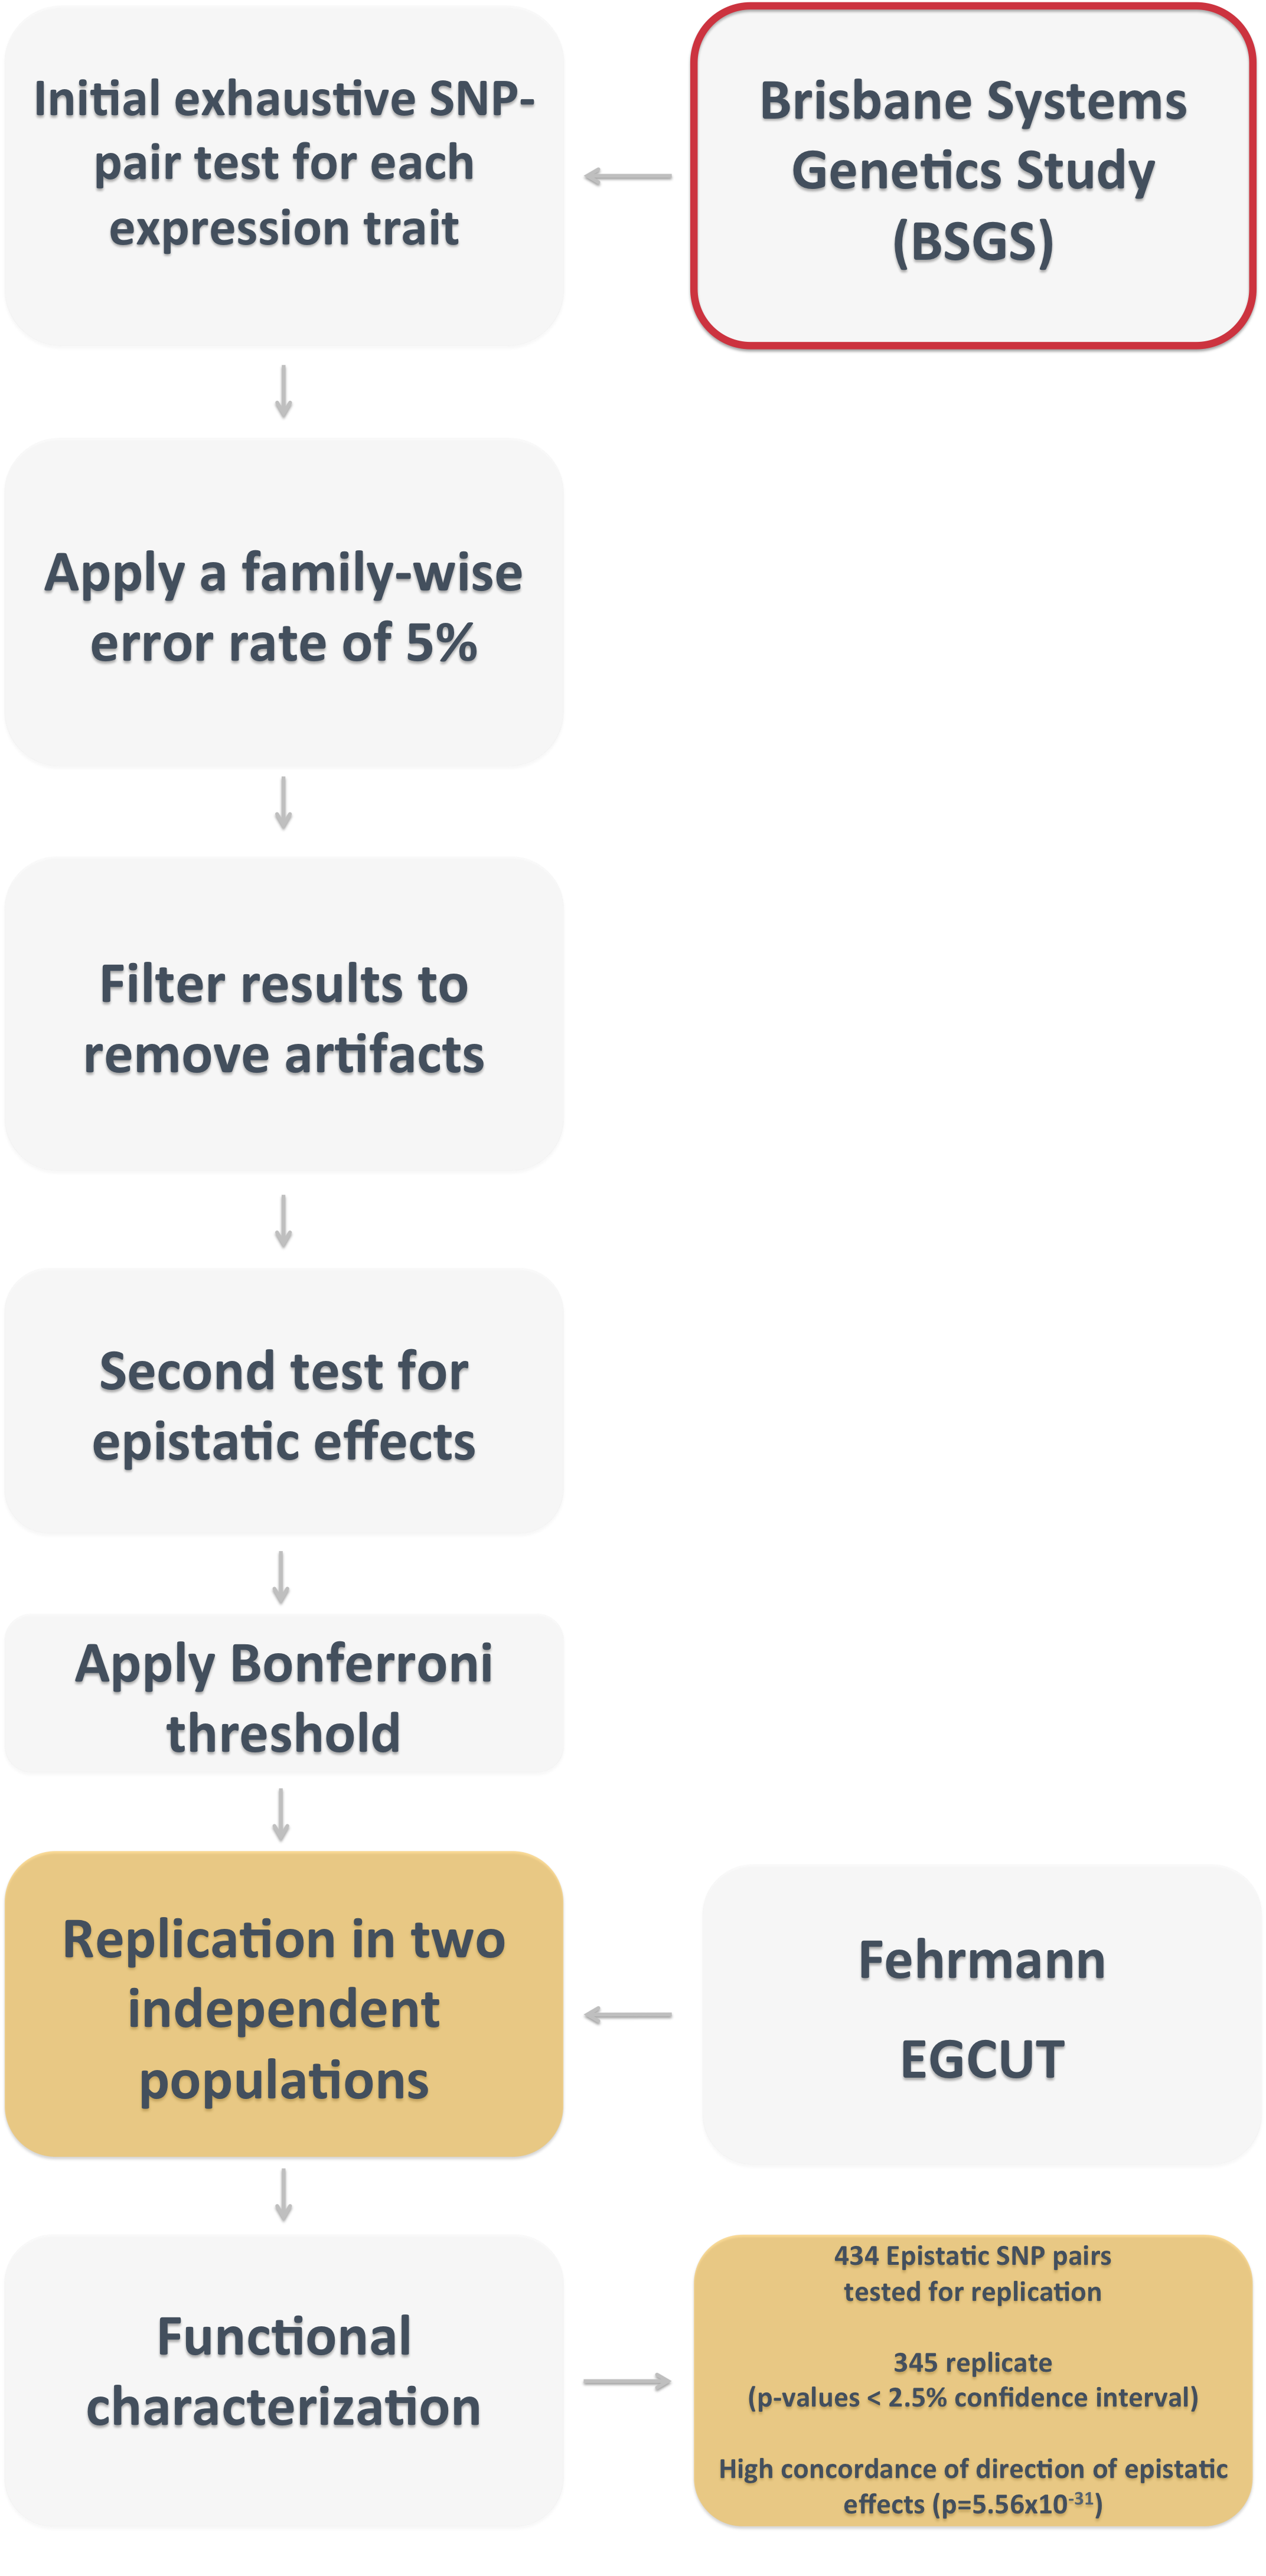
\includegraphics[height=7cm]{images/methods2.png} \\
\end{center}
\end{frame}

\begin{frame}
\begin{columns}[c]
\column{.5\textwidth}

\includegraphics[width=4.5cm]{images/BSGS.png} \\
\column{.5\textwidth} 
\begin{itemize}
\item 846 healthy individuals 
\vspace{0.3cm}
\item 528,509 autosomal SNPs
\vspace{0.3cm}
\item RNA measued for peripheral blood (Illumina HT-12v4.0)
\vspace{0.3cm}
\item Expression levels for 7,339 probes 
\end{itemize}
\end{columns}
\end{frame}

\begin{frame}
\begin{center}
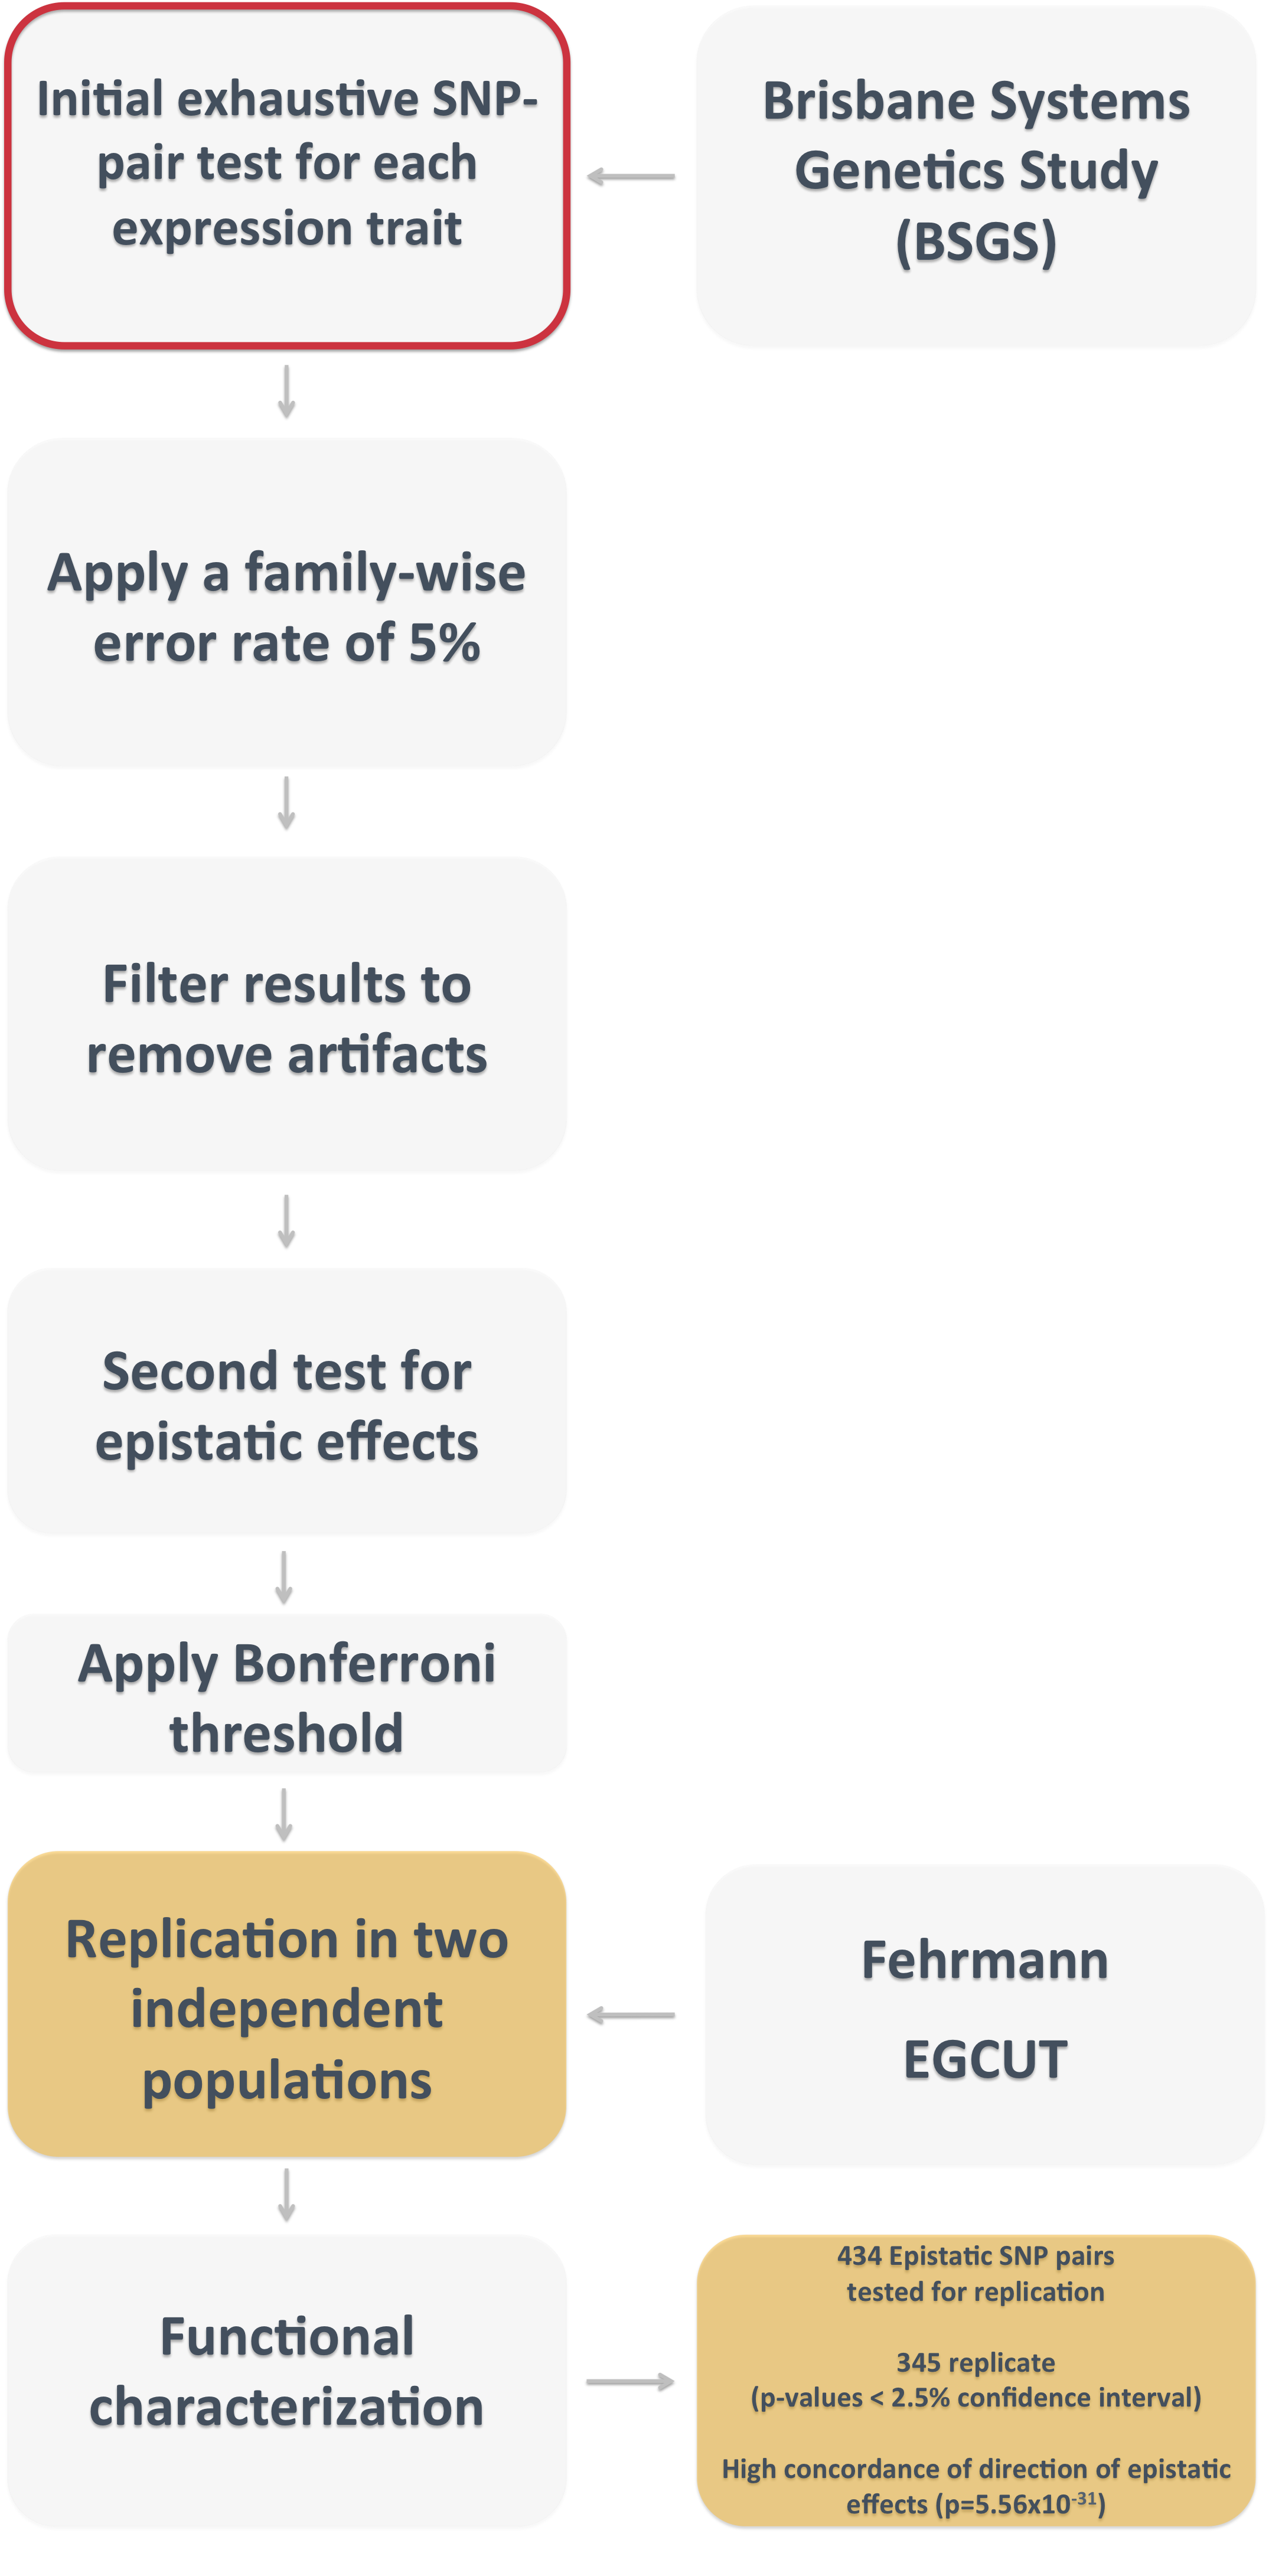
\includegraphics[height=7cm]{images/methods3.png} \\
\end{center}
\end{frame}

\begin{frame}
\begin{columns}[c]
\column{.5\textwidth}
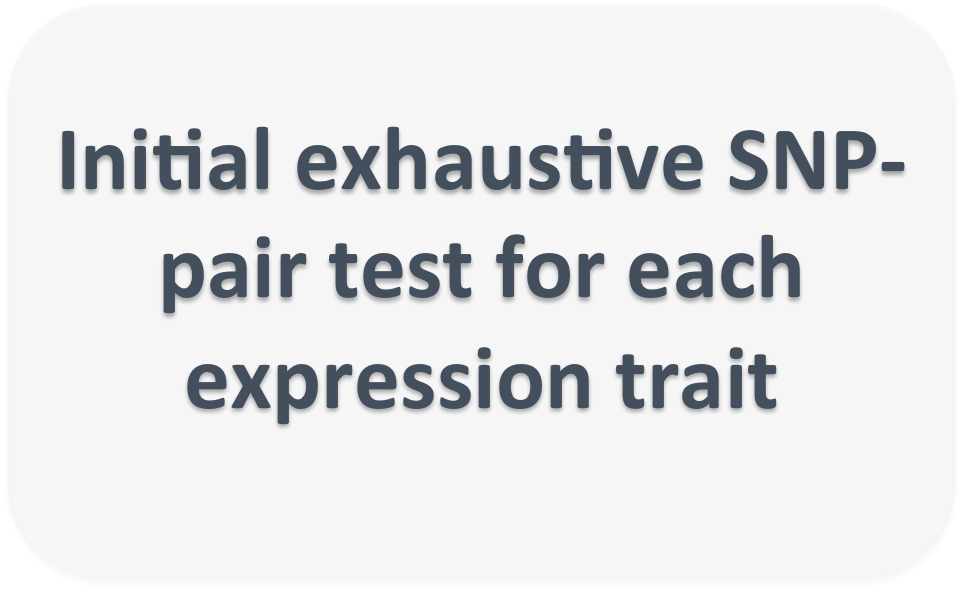
\includegraphics[width=4.5cm]{images/exhaustive.png} \\
\column{.5\textwidth} 
\begin{itemize}
\item Exhaustive SNP x SNP testing for each probe
\vspace{0.3cm}
\item epiGPU software and GPU clusters
\vspace{0.3cm}
\item 8 d.f. F-test 
\vspace{0.3cm}
\item Over quadrillion tests  
\end{itemize}
\end{columns}
\end{frame}

\begin{frame}
\begin{center}
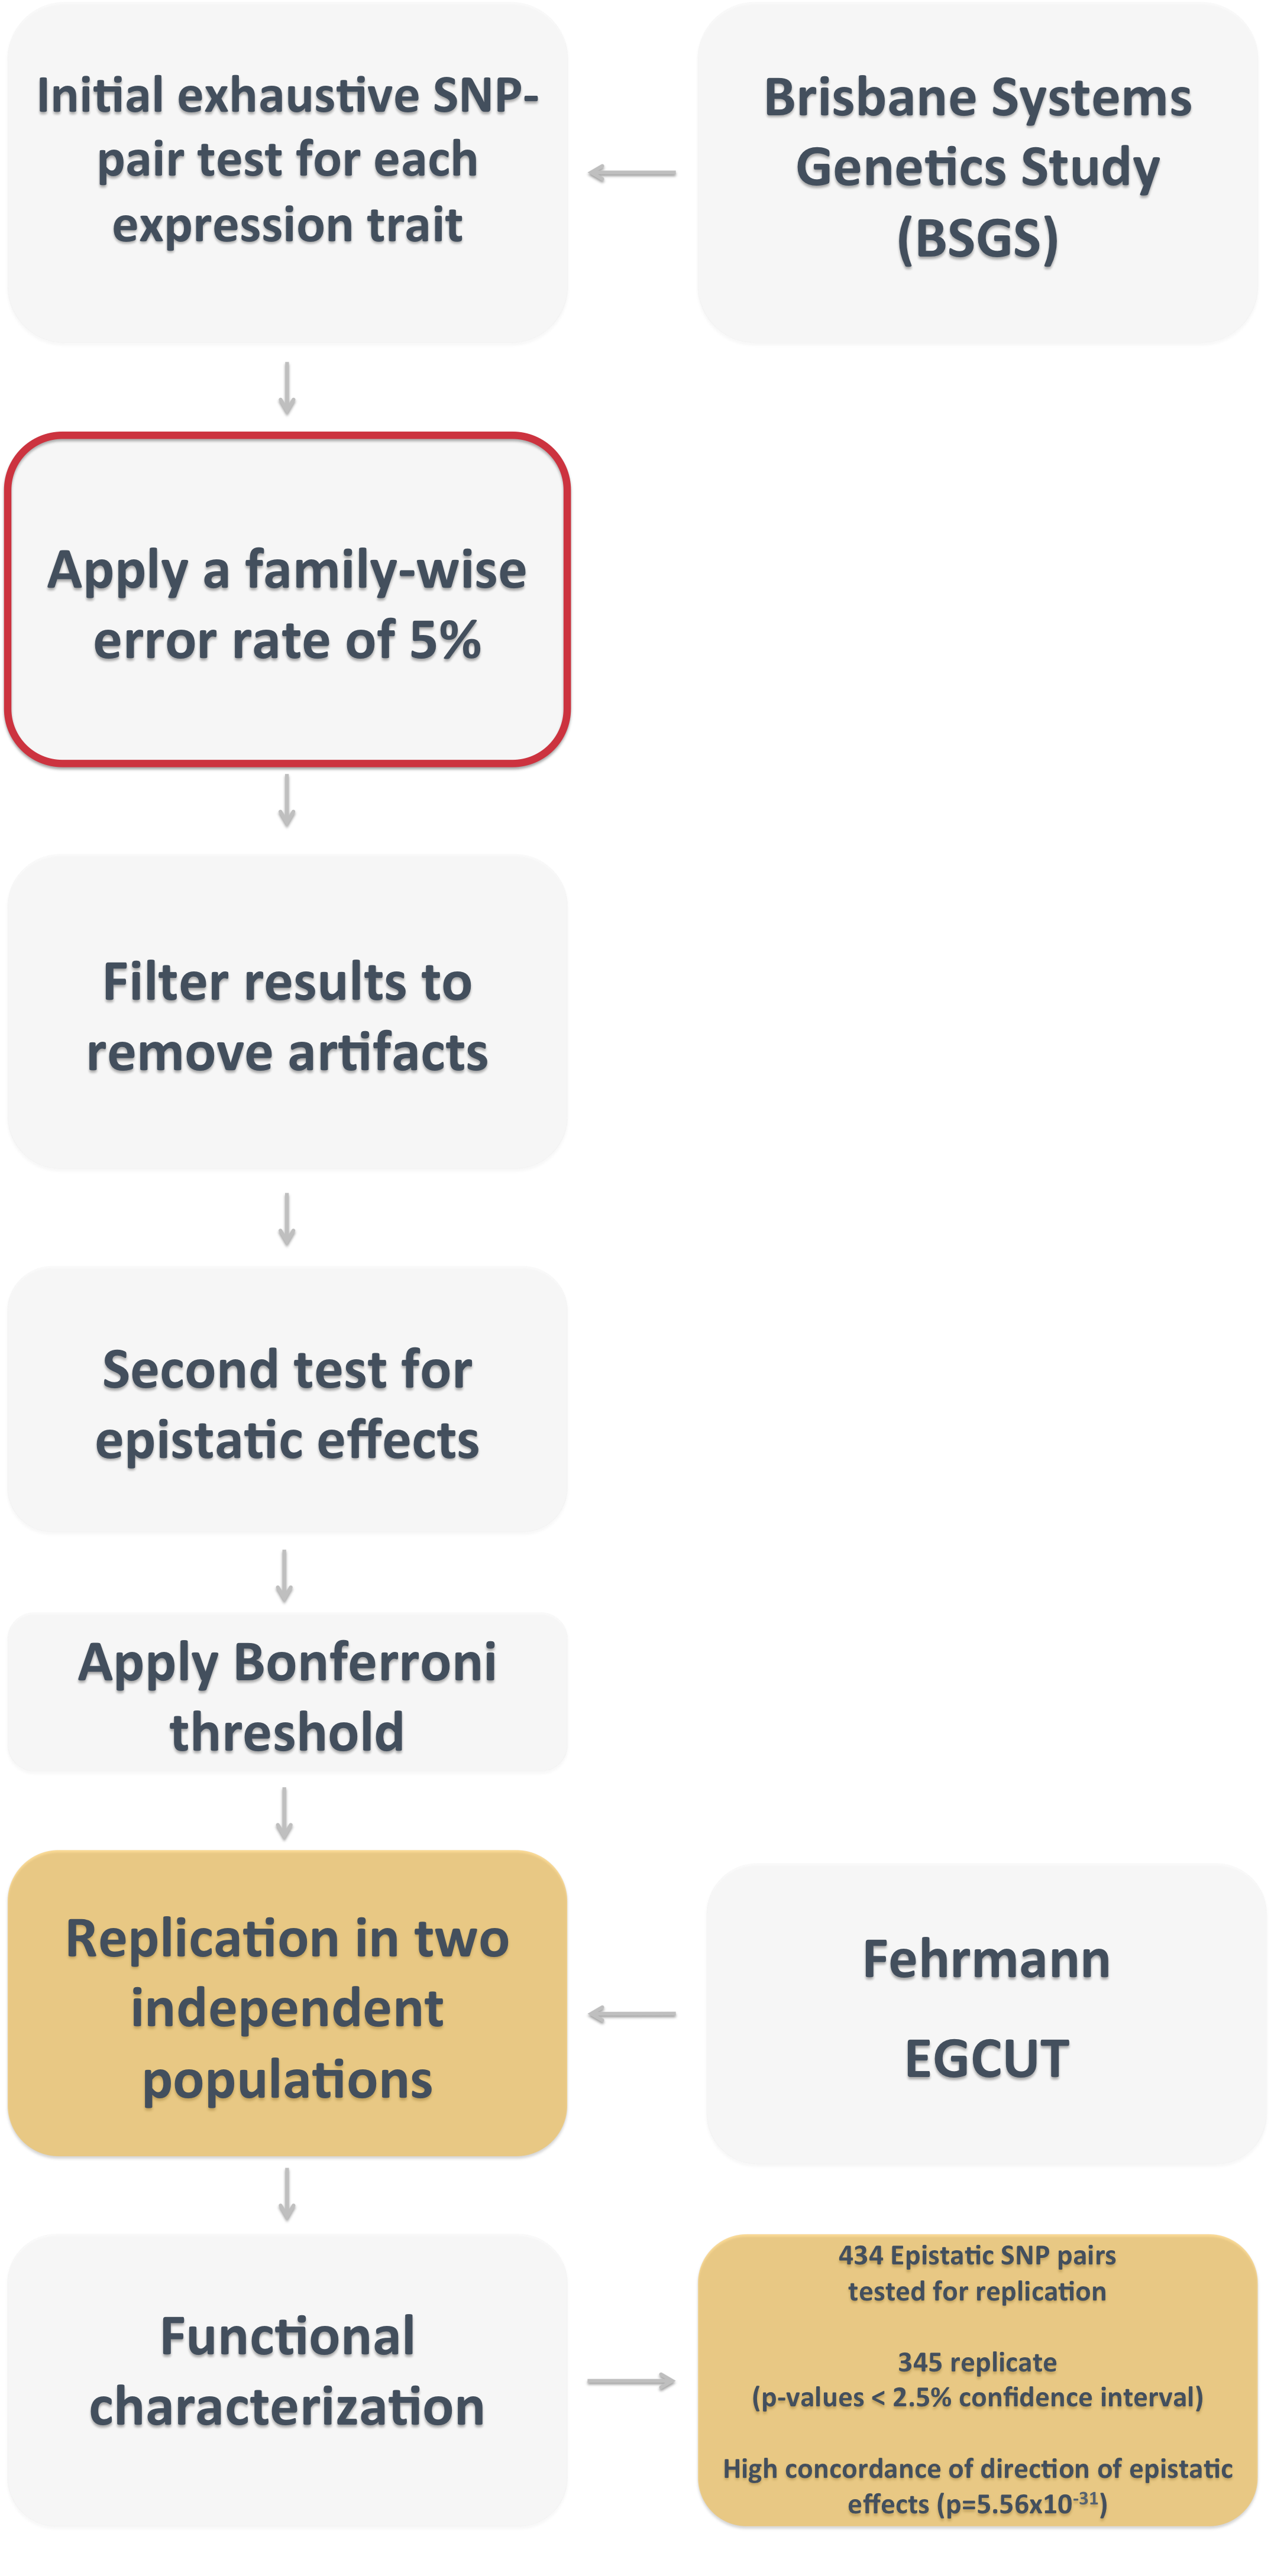
\includegraphics[height=7cm]{images/methods4.png} \\
\end{center}
\end{frame}

\begin{frame}
\begin{columns}[c]
\column{.5\textwidth}

\includegraphics[width=4.5cm]{images/fam_wise.pdf} \\
\column{.5\textwidth} 
\begin{itemize}
\item Permutation and bonferoni used to give 5\% FWER
\vspace{0.2cm} 
\item Permutation: Single probe FWER;  $T*= 2.13x10^{-12}$ 
\vspace{0.2cm} 
\item Correct for 7,339 probes
\vspace{0.2cm} 
\item Experiment wide FWER; $T*/7,339=2.91x10^{-16}$  
\end{itemize}
\end{columns}
\end{frame}

\begin{frame}
\begin{center}
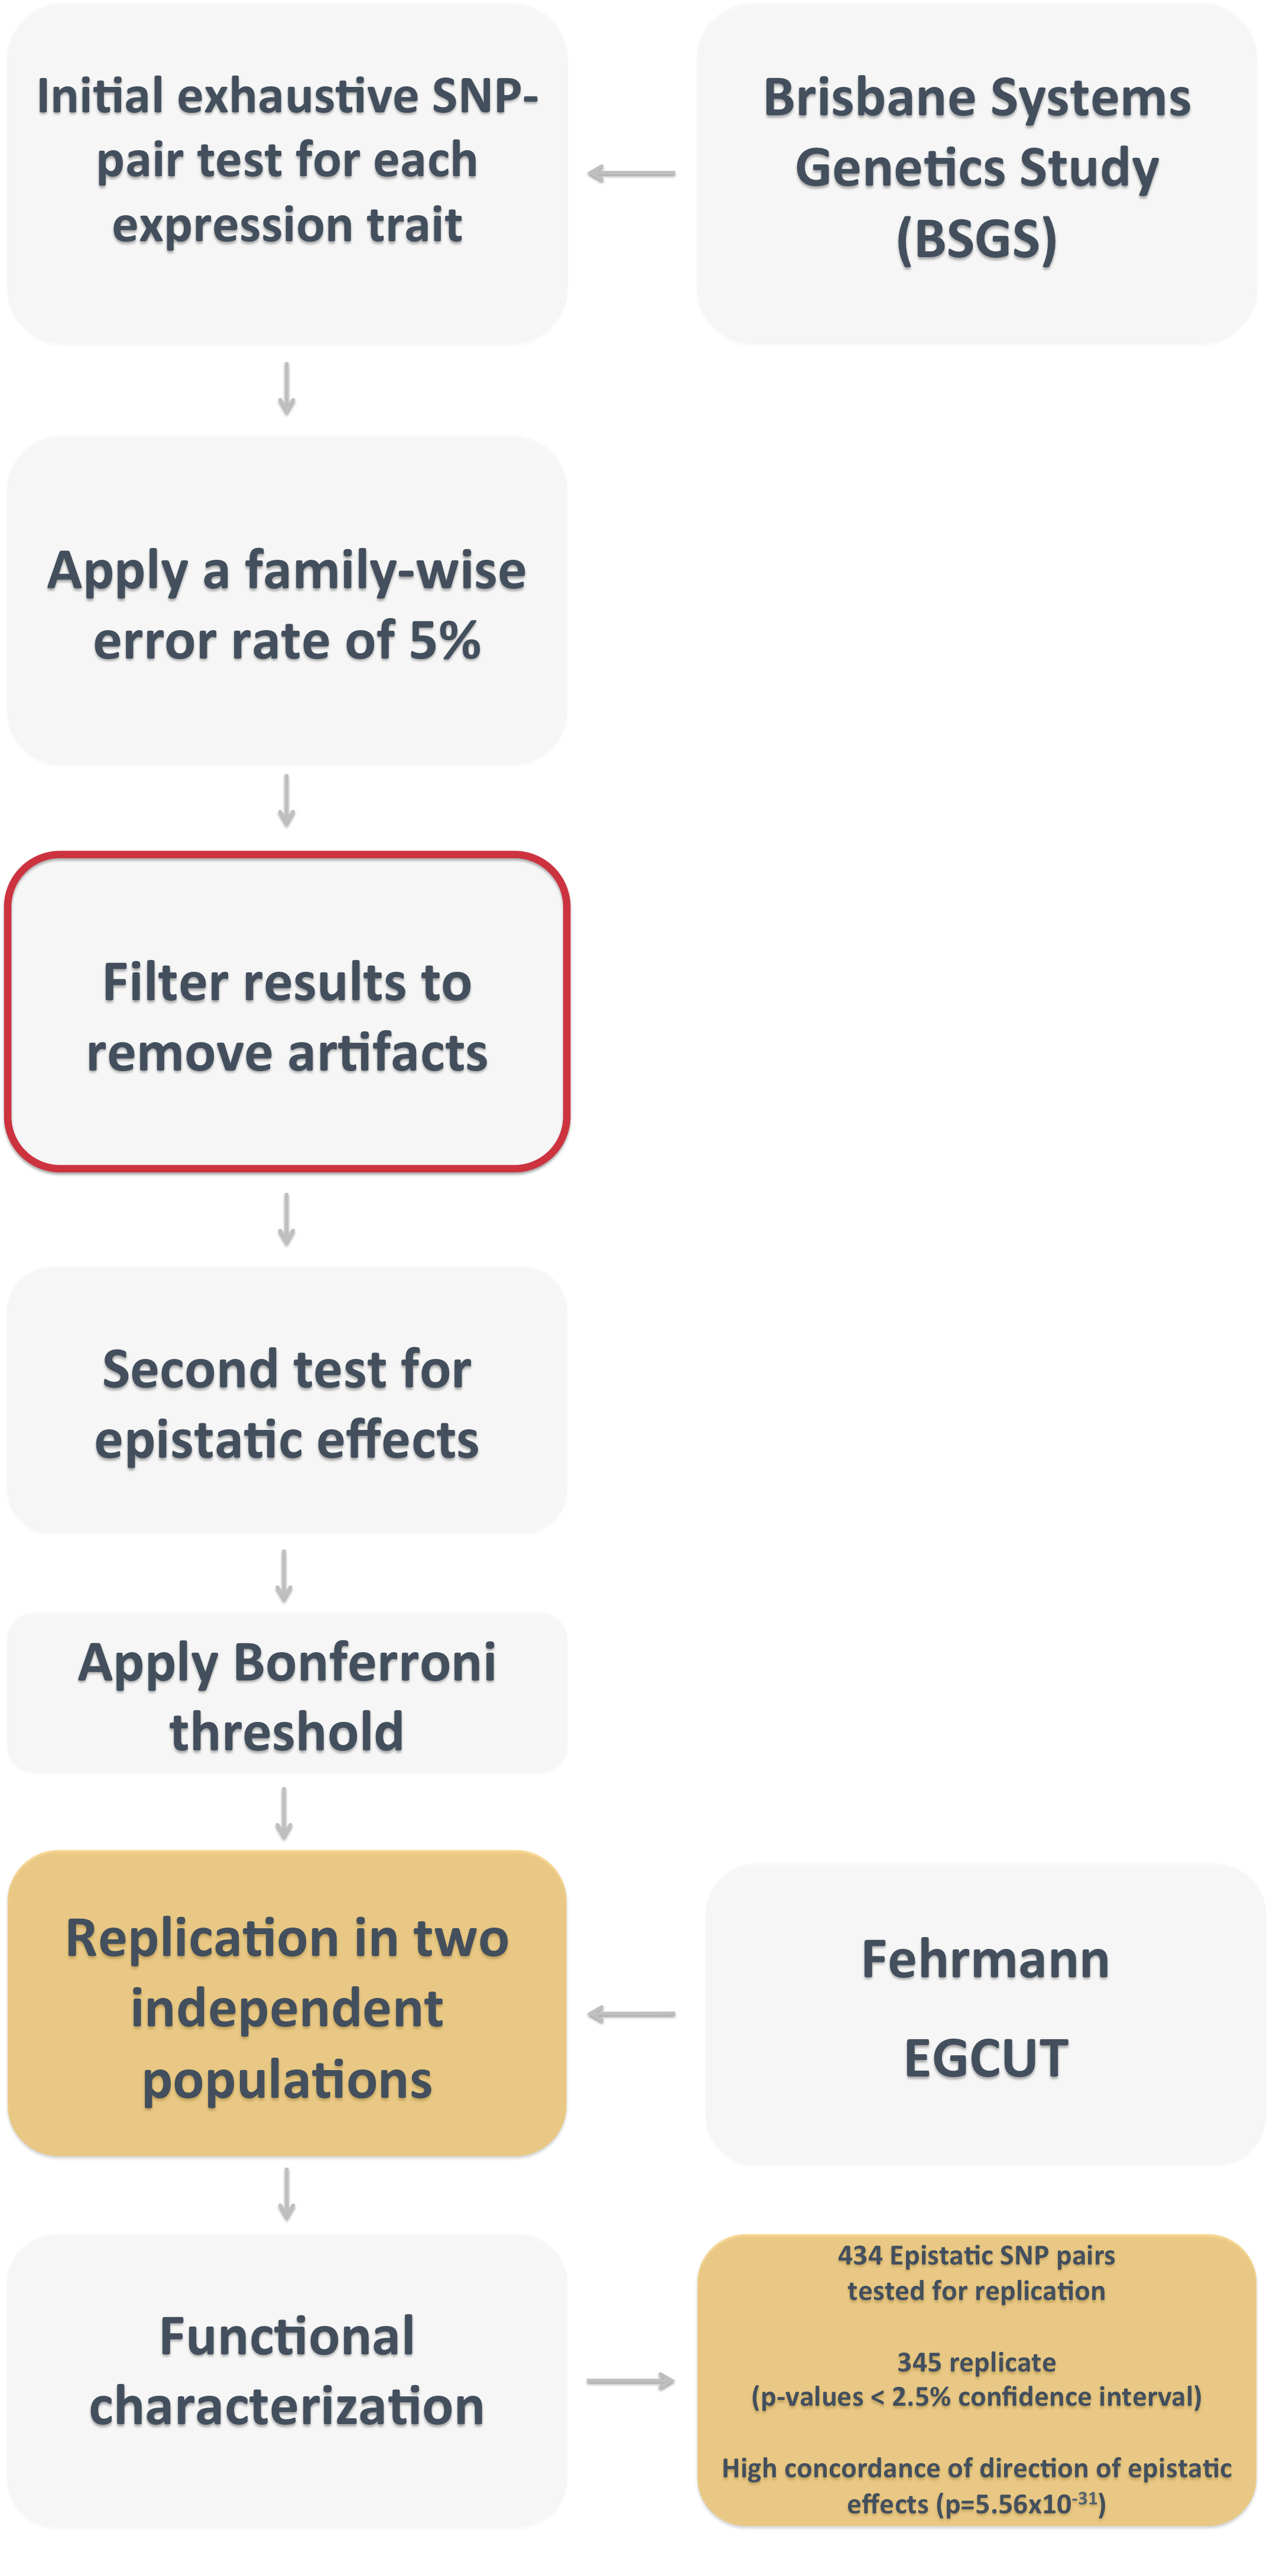
\includegraphics[height=7cm]{images/methods5.png} \\
\end{center}
\end{frame}

\begin{frame}
\begin{columns}[c]
\column{.5\textwidth}

\includegraphics[width=4.5cm]{images/filter.png} \\
\column{.5\textwidth} 
\begin{itemize}
\item For SNP pairs that passed the $2.91x10^{-16}$ threshold
\vspace{0.1cm} 
\item All 9 genotypes classes present
\vspace{0.1cm} 
\item Minimum class size of 5
\vspace{0.1cm} 
\item No LD between SNP pairs ($r^2 < 0.1$ and $D'^2 < 0.1$)
\vspace{0.1cm} 
\item No single loci additive or dominance effects
\vspace{0.1cm} 
\item 11,155 pairs carried forward
\end{itemize}
\end{columns}
\end{frame}

\begin{frame}
\begin{center}
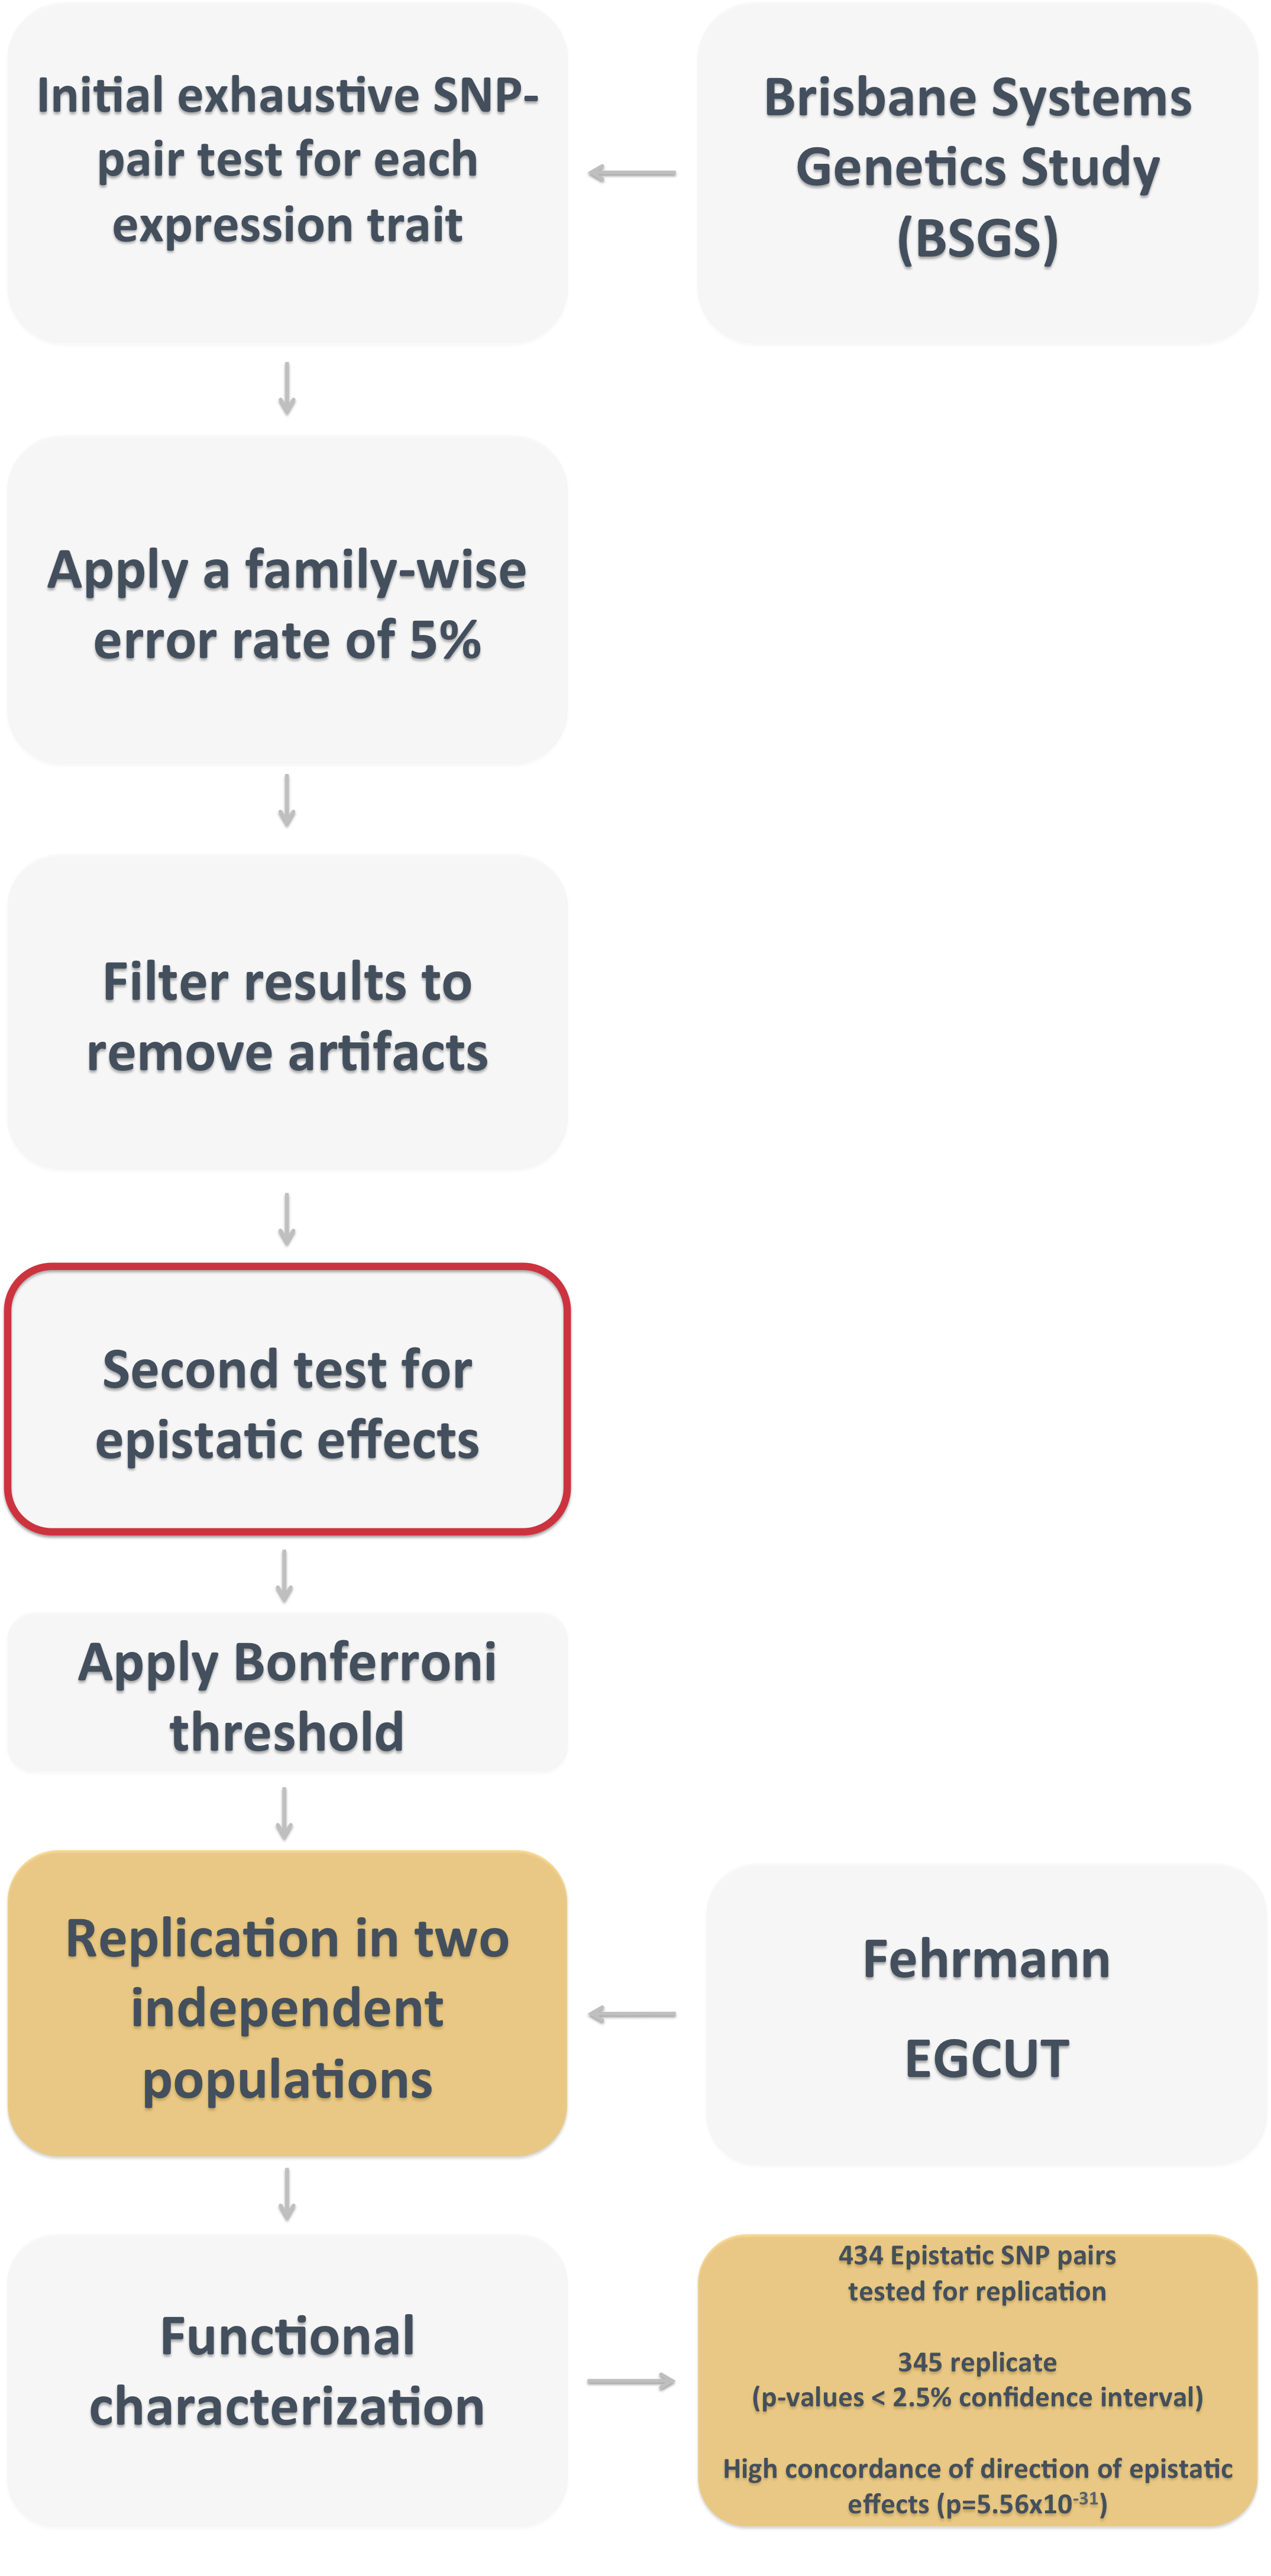
\includegraphics[height=7cm]{images/methods6.png} \\
\end{center}
\end{frame}

\begin{frame}
\begin{columns}[c]
\column{.5\textwidth}

\includegraphics[width=4.5cm]{images/second.png} \\
\column{.5\textwidth} 
\begin{itemize}
\item Nested ANOVA for 11,155 pairs 
\vspace{0.2cm} 
\item Contrasts full genetic (8 d.f.) vs marginal effects (4 d.f)
\vspace{0.2cm} 
\item Thus, testing for the contribution of epistatic variance 
\end{itemize}
\end{columns}
\end{frame}

\begin{frame}
\begin{center}
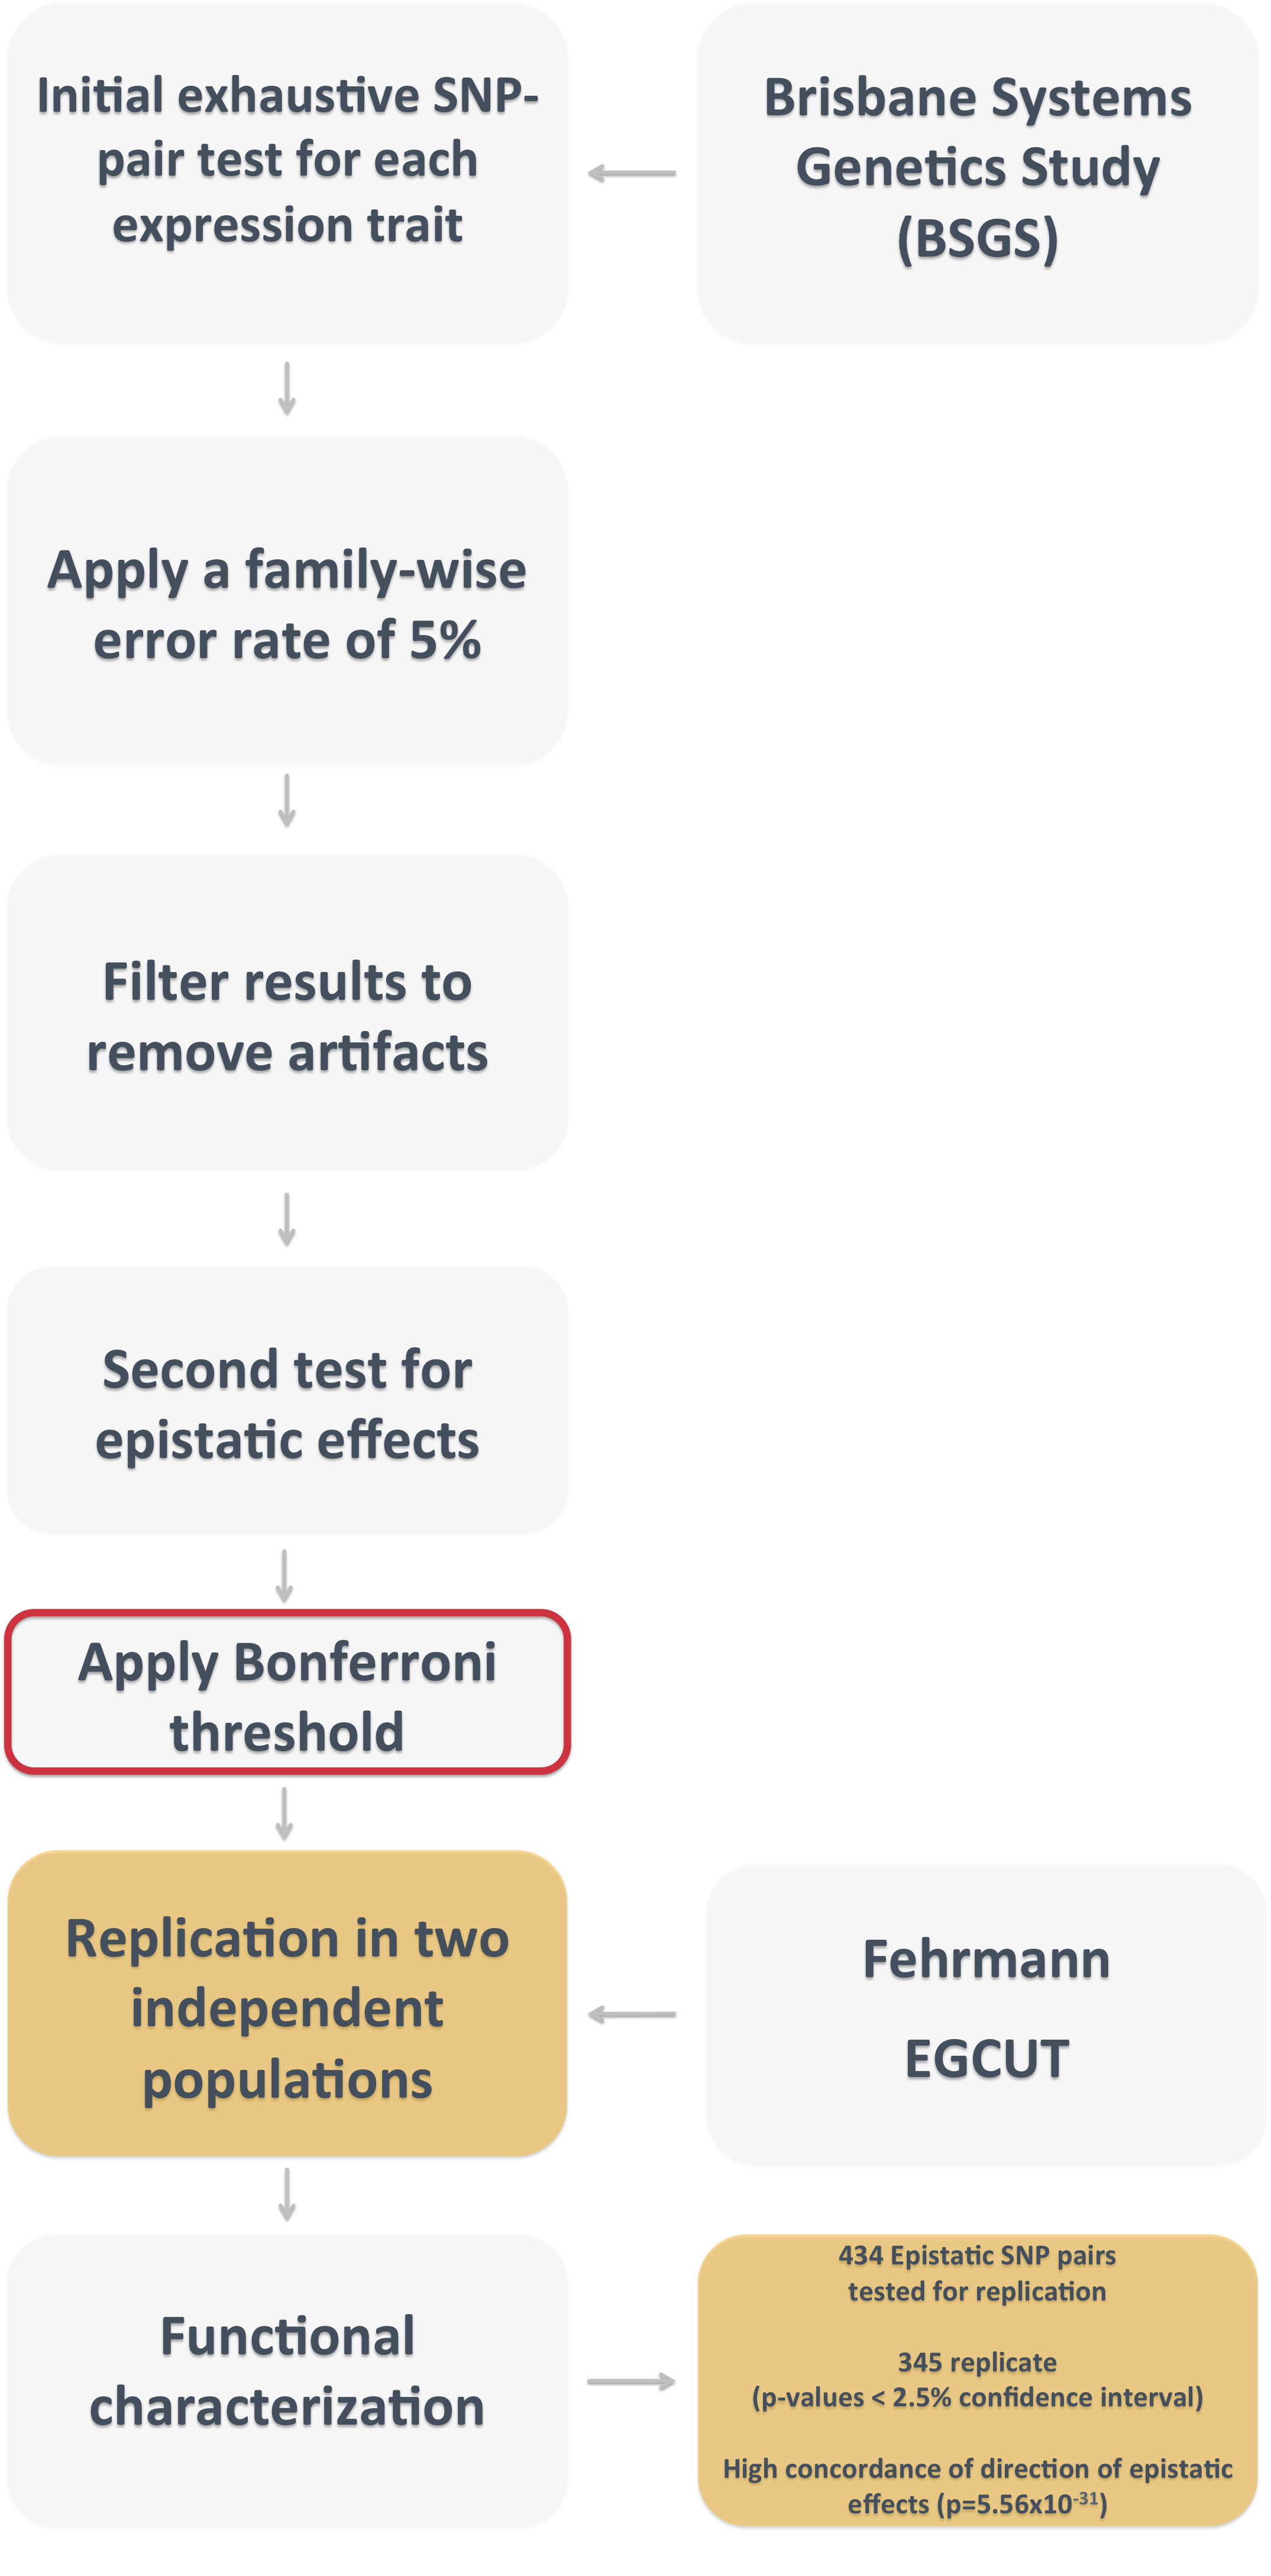
\includegraphics[height=7cm]{images/methods7.png} \\
\end{center}
\end{frame}

\begin{frame}
\begin{columns}[c]
\column{.5\textwidth}

\includegraphics[width=4.5cm]{images/bonf.png} \\
\column{.5\textwidth} 
\begin{itemize}
\item Epistatic effects significant at $p < 0.05/11,155 = 4.48x10^{-6}$
\vspace{0.2cm} 
\item 501 SNP pairs with significant interaction terms 
\end{itemize}
\end{columns}
\end{frame}

\begin{frame}
\begin{center}
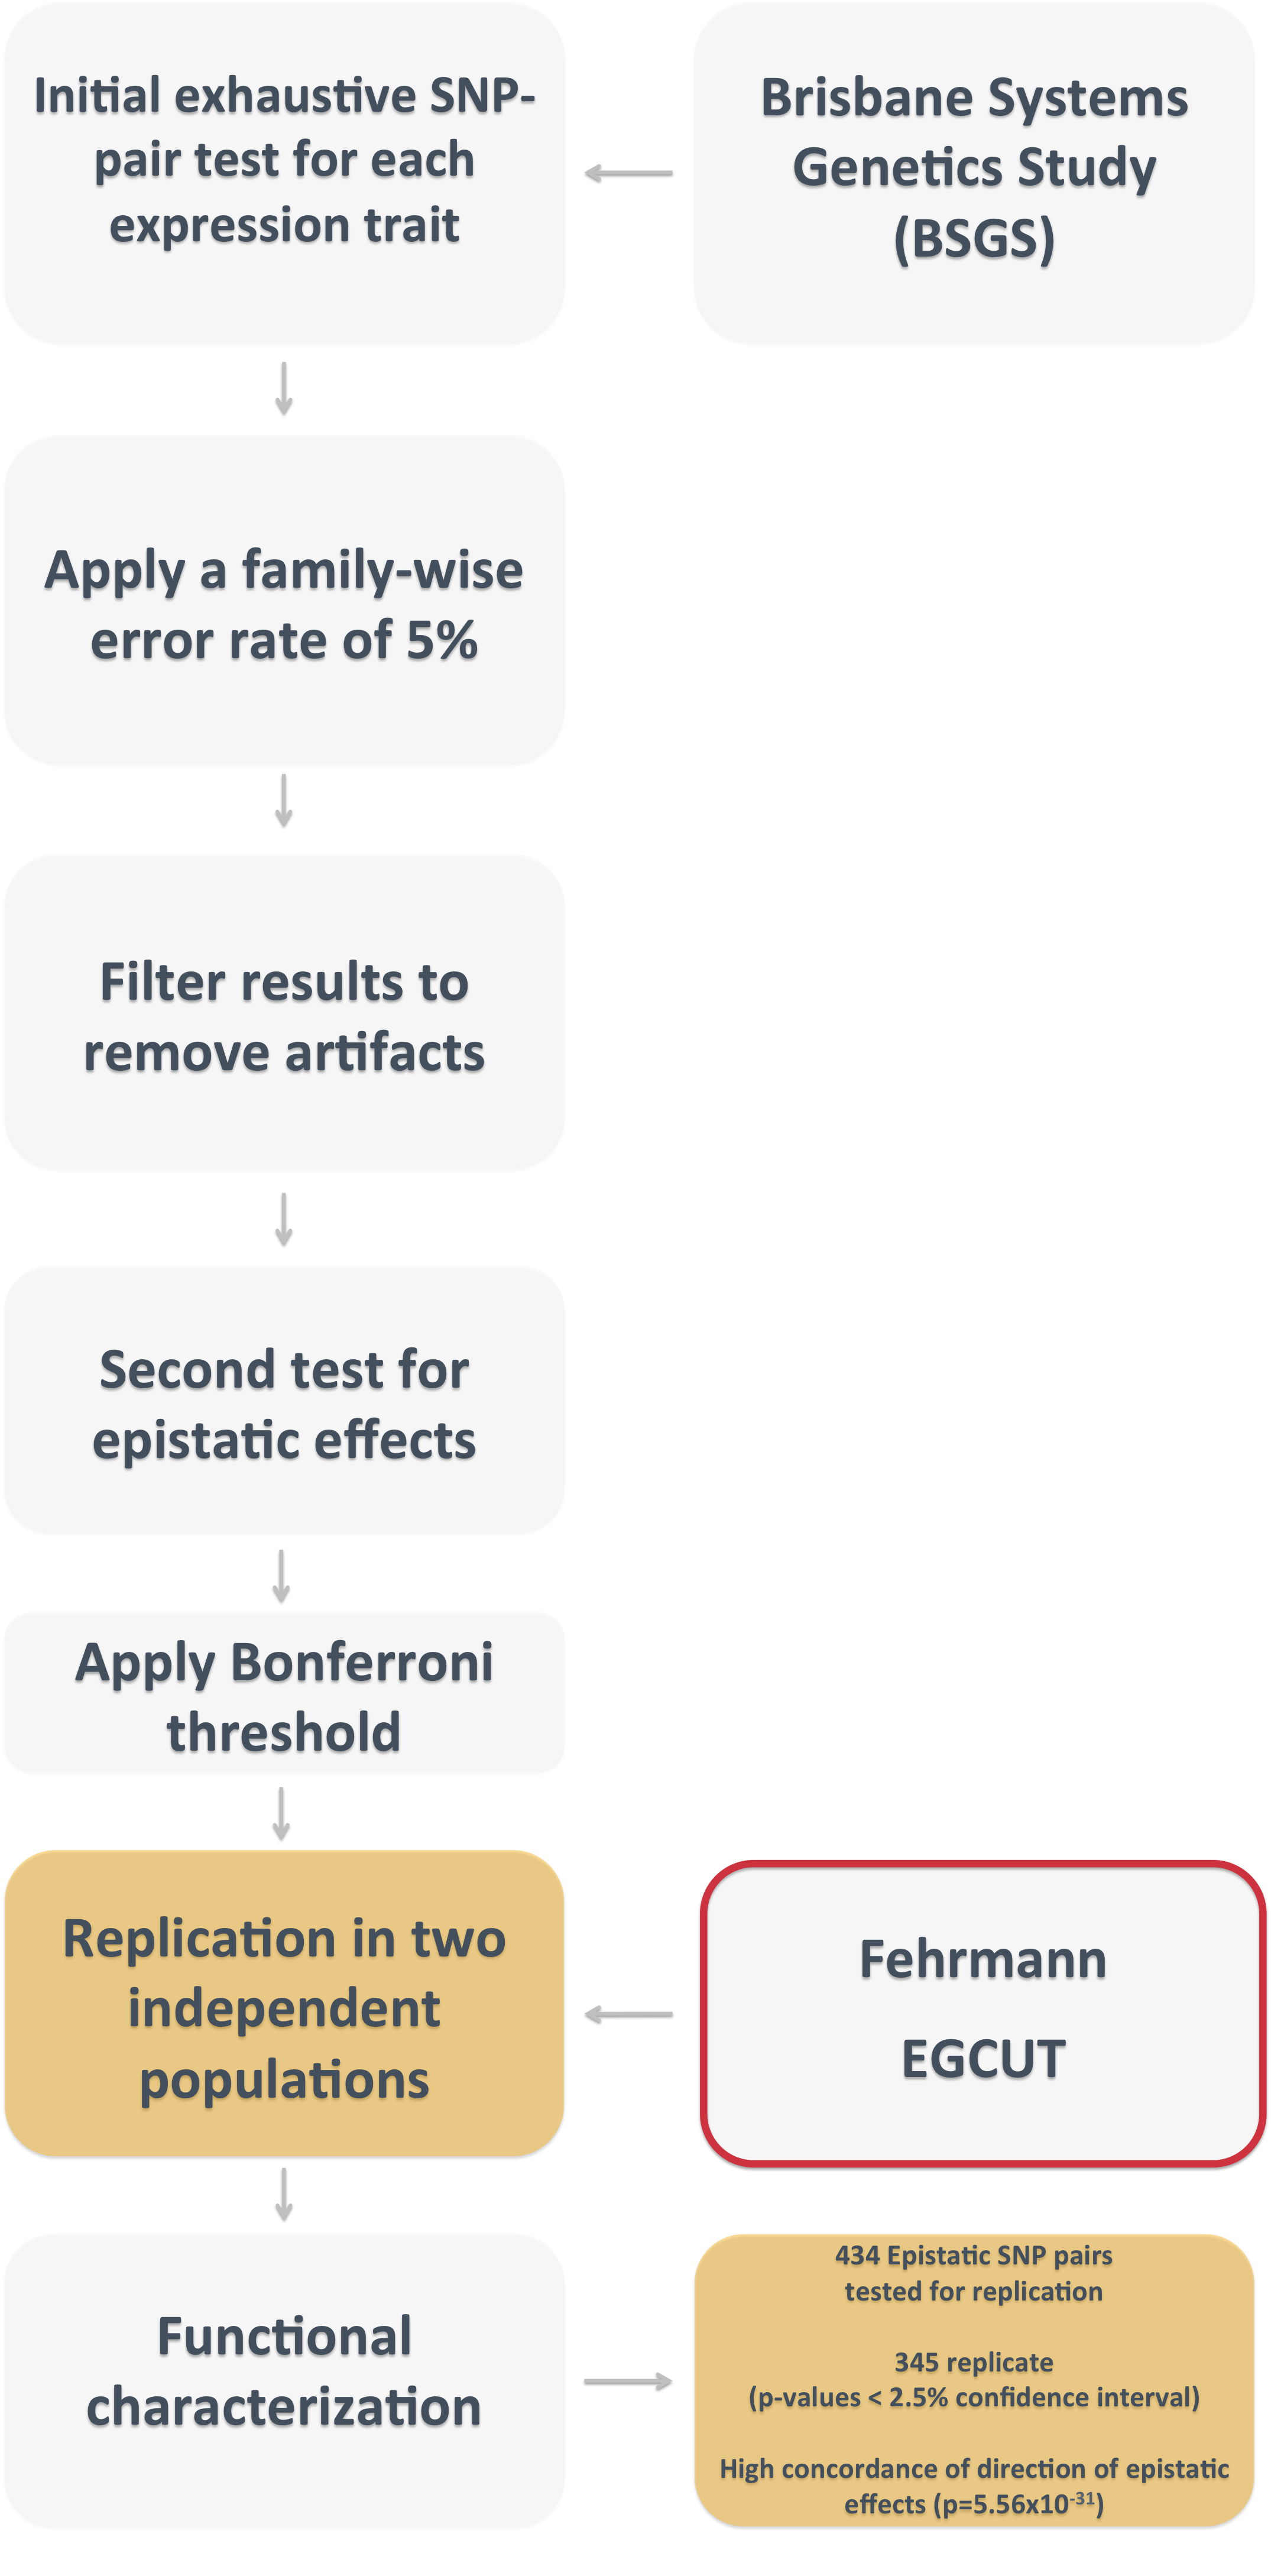
\includegraphics[height=7cm]{images/methods8.png} \\
\end{center}
\end{frame}

\begin{frame}
\begin{columns}[c]
\column{.5\textwidth}

\includegraphics[width=4.5cm]{images/rep1.png} \\
\column{.5\textwidth} 
Fehrmann
\begin{itemize}
\item 1,240 individuals (Netherlands) 
\end{itemize}
\vspace{0.3cm}
EGCUT
\begin{itemize}
\item 891 individuals (Estonian)
\vspace{0.3cm}
\item RNA measued for peripheral blood (Illumina HT-12v3.0)
\vspace{0.1cm} 
\item Genotyped with Illumina arrays
\end{itemize}
\end{columns}
\end{frame}

\begin{frame}
\begin{center}
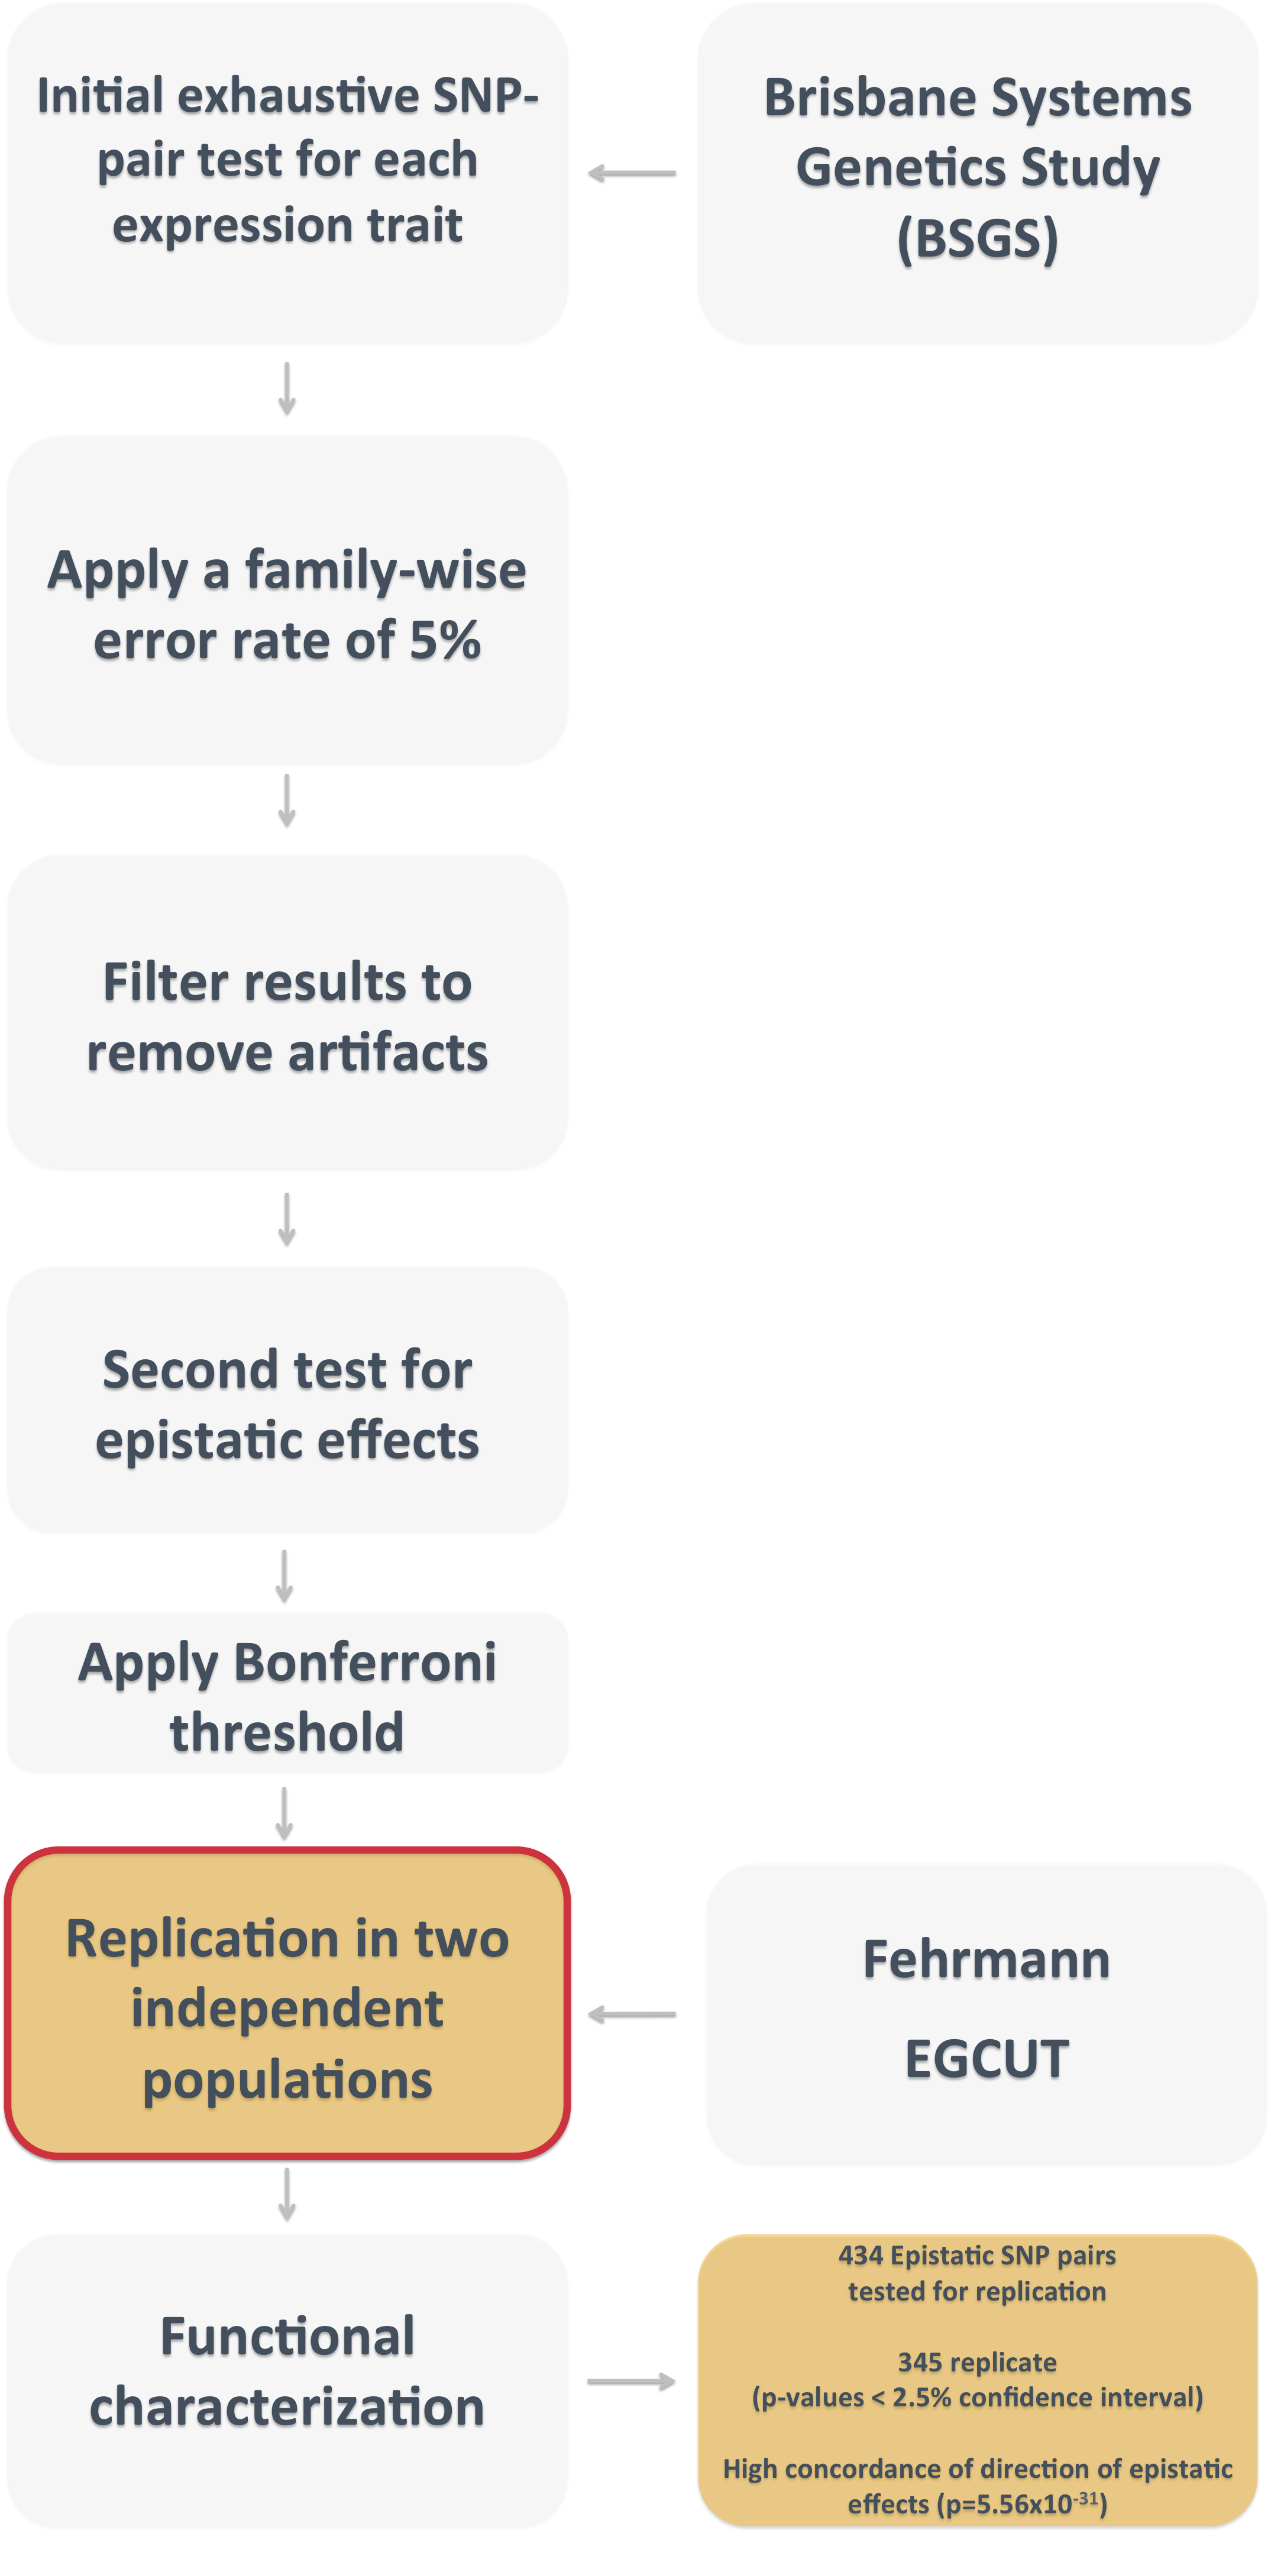
\includegraphics[height=7cm]{images/methods9.png} \\
\end{center}
\end{frame}

\begin{frame}
\begin{columns}[c]
\column{.5\textwidth}
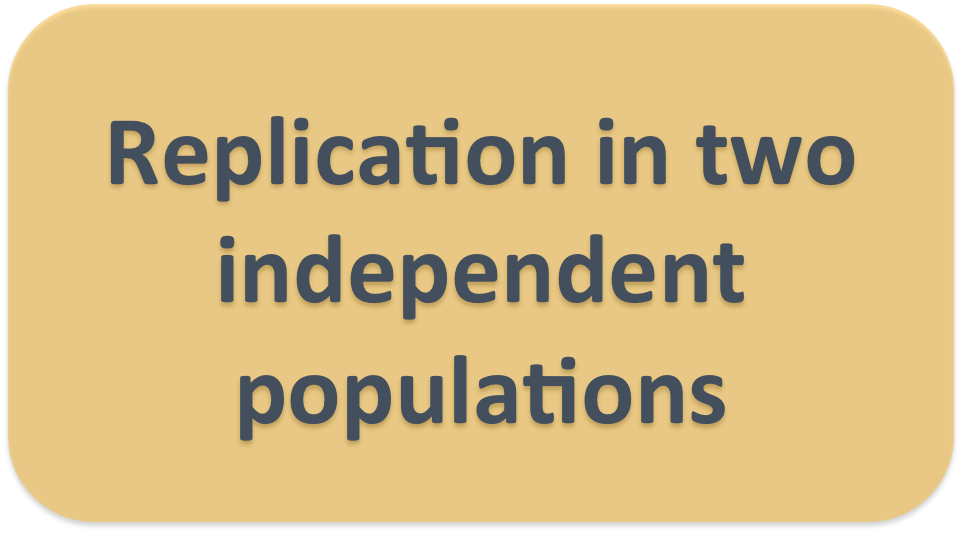
\includegraphics[width=4.5cm]{images/rep2.png} \\
\column{.5\textwidth} 
\begin{itemize}
\item Replication of 501 epistatic hits using two independent cohorts 
\vspace{0.1cm}
\item Same filtering criteria
\vspace{0.1cm}
\item 434 pairs which could be tested in both cohorts 
\end{itemize}
\end{columns}
\end{frame}

\begin{frame}
\begin{center}
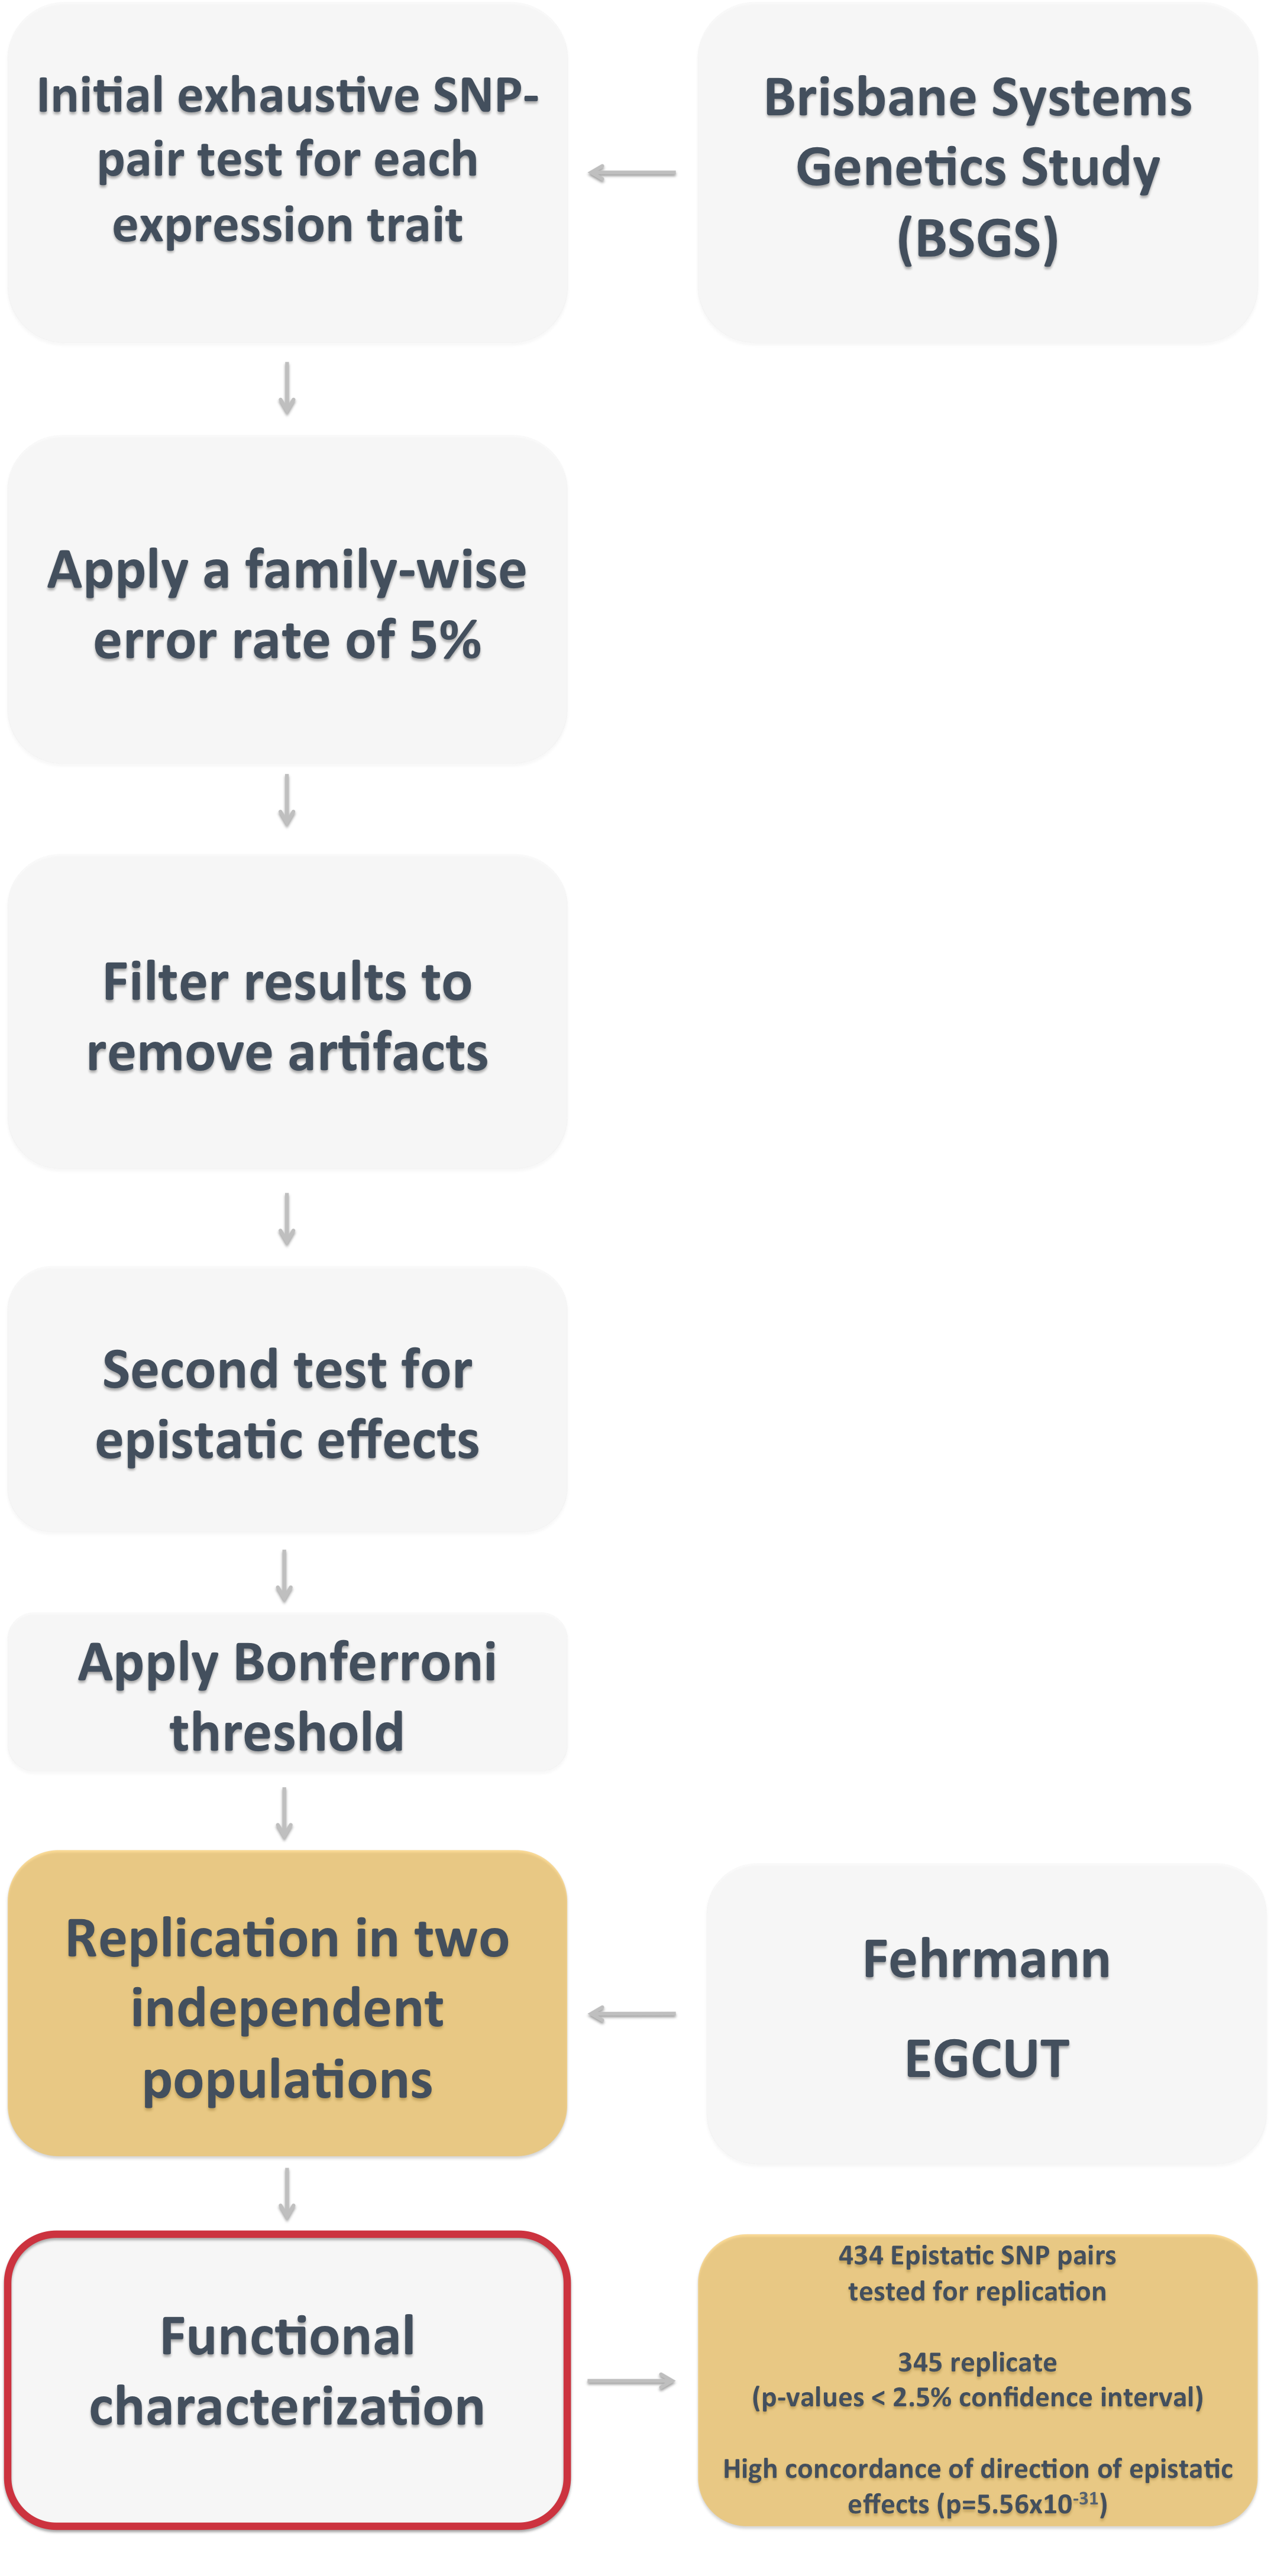
\includegraphics[height=7cm]{images/methods10.png} \\
\end{center}
\end{frame}

\begin{frame}
\begin{columns}[c]
\column{.5\textwidth}
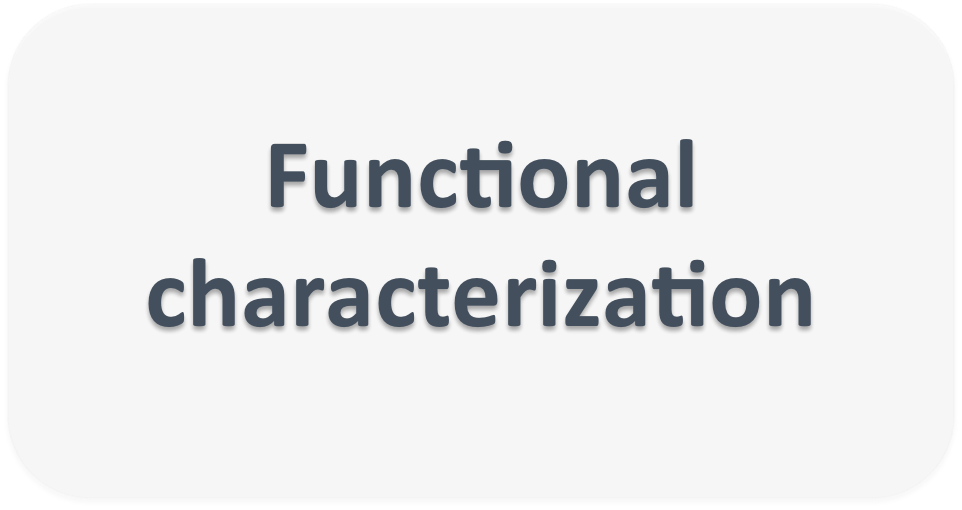
\includegraphics[width=4.5cm]{images/func.png} \\
\column{.5\textwidth} 
Analyses to elucidate possible functional mechanisms
\begin{itemize}
\item Non-synonymous mutations
\vspace{0.1cm}
\item GWAS and known eQTL overlap
\vspace{0.1cm}
\item Genome segmentation
\vspace{0.1cm}
\item Chromosome interactions
\vspace{0.1cm}
\item Tissue specific transcription regions
\end{itemize}
\end{columns}
\end{frame}

%%%%%%%%%%%%%%%%%%%%%%%%%%%%%%%%%%%%%%%%%%%%%%%%%%%%%%%%
%%%%%%%%%%%%%%%%%%%%%%%%%%%%%%%%%%%%%%%%%%%%%%%%%%%%%%%%

\section{Results}
\subsection{}
\begin{frame}{Q-Q plots of interaction p-values from replication}
\begin{columns}[c]
\column{.5\textwidth}
The top panel shows all 434 discovery SNPs that were tested for interactions. \\
\vspace{0.3cm}
The bottom panel shows the same data as the top panel but excluding the 30 most significant interactions \\
\vspace{0.3cm}
Matched direction of epistatic effects $p=5.56x10^{-31}$ 
\column{.5\textwidth} 
\begin{center}
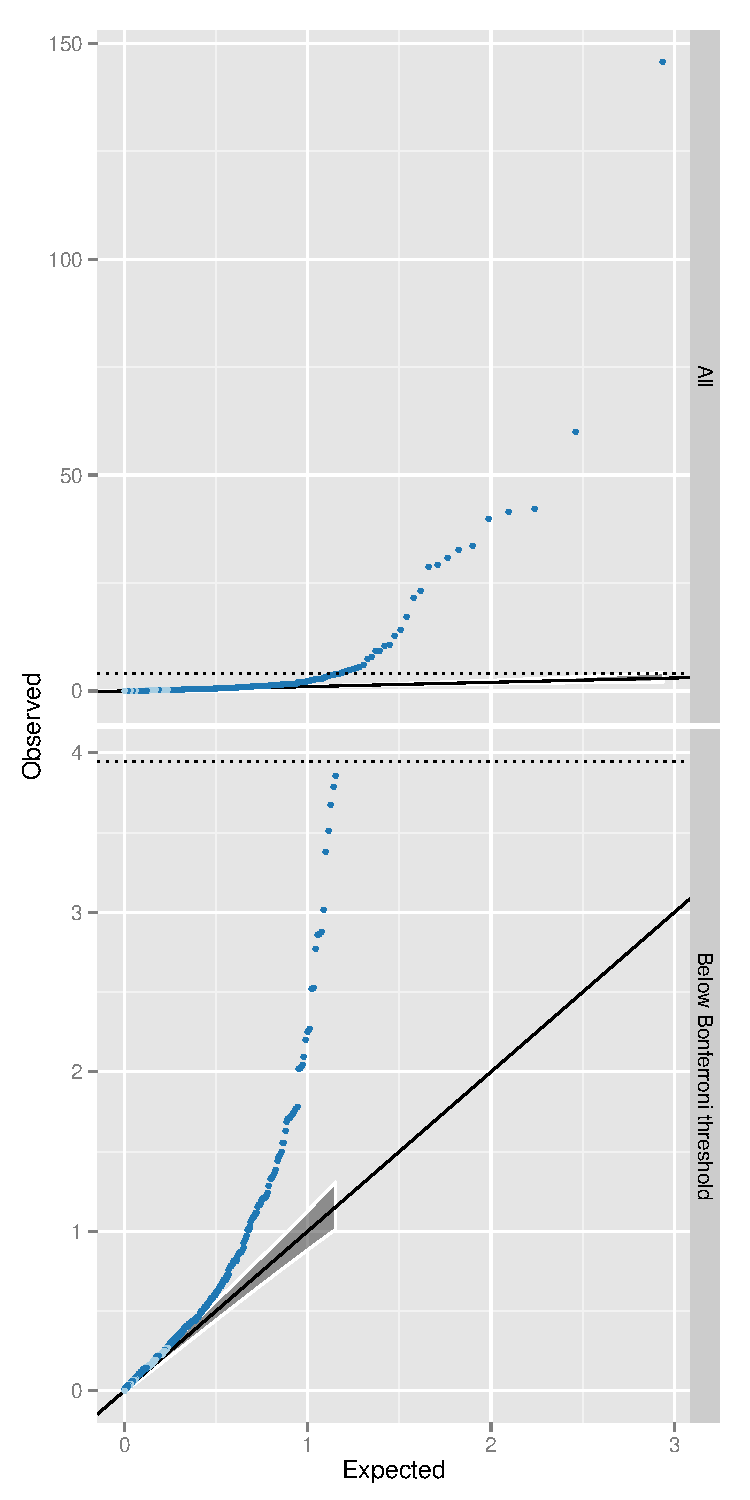
\includegraphics[height=6.5cm]{images/qqMeta.pdf} \\
\end{center}
\end{columns}
\end{frame}

\begin{frame}
\begin{center}
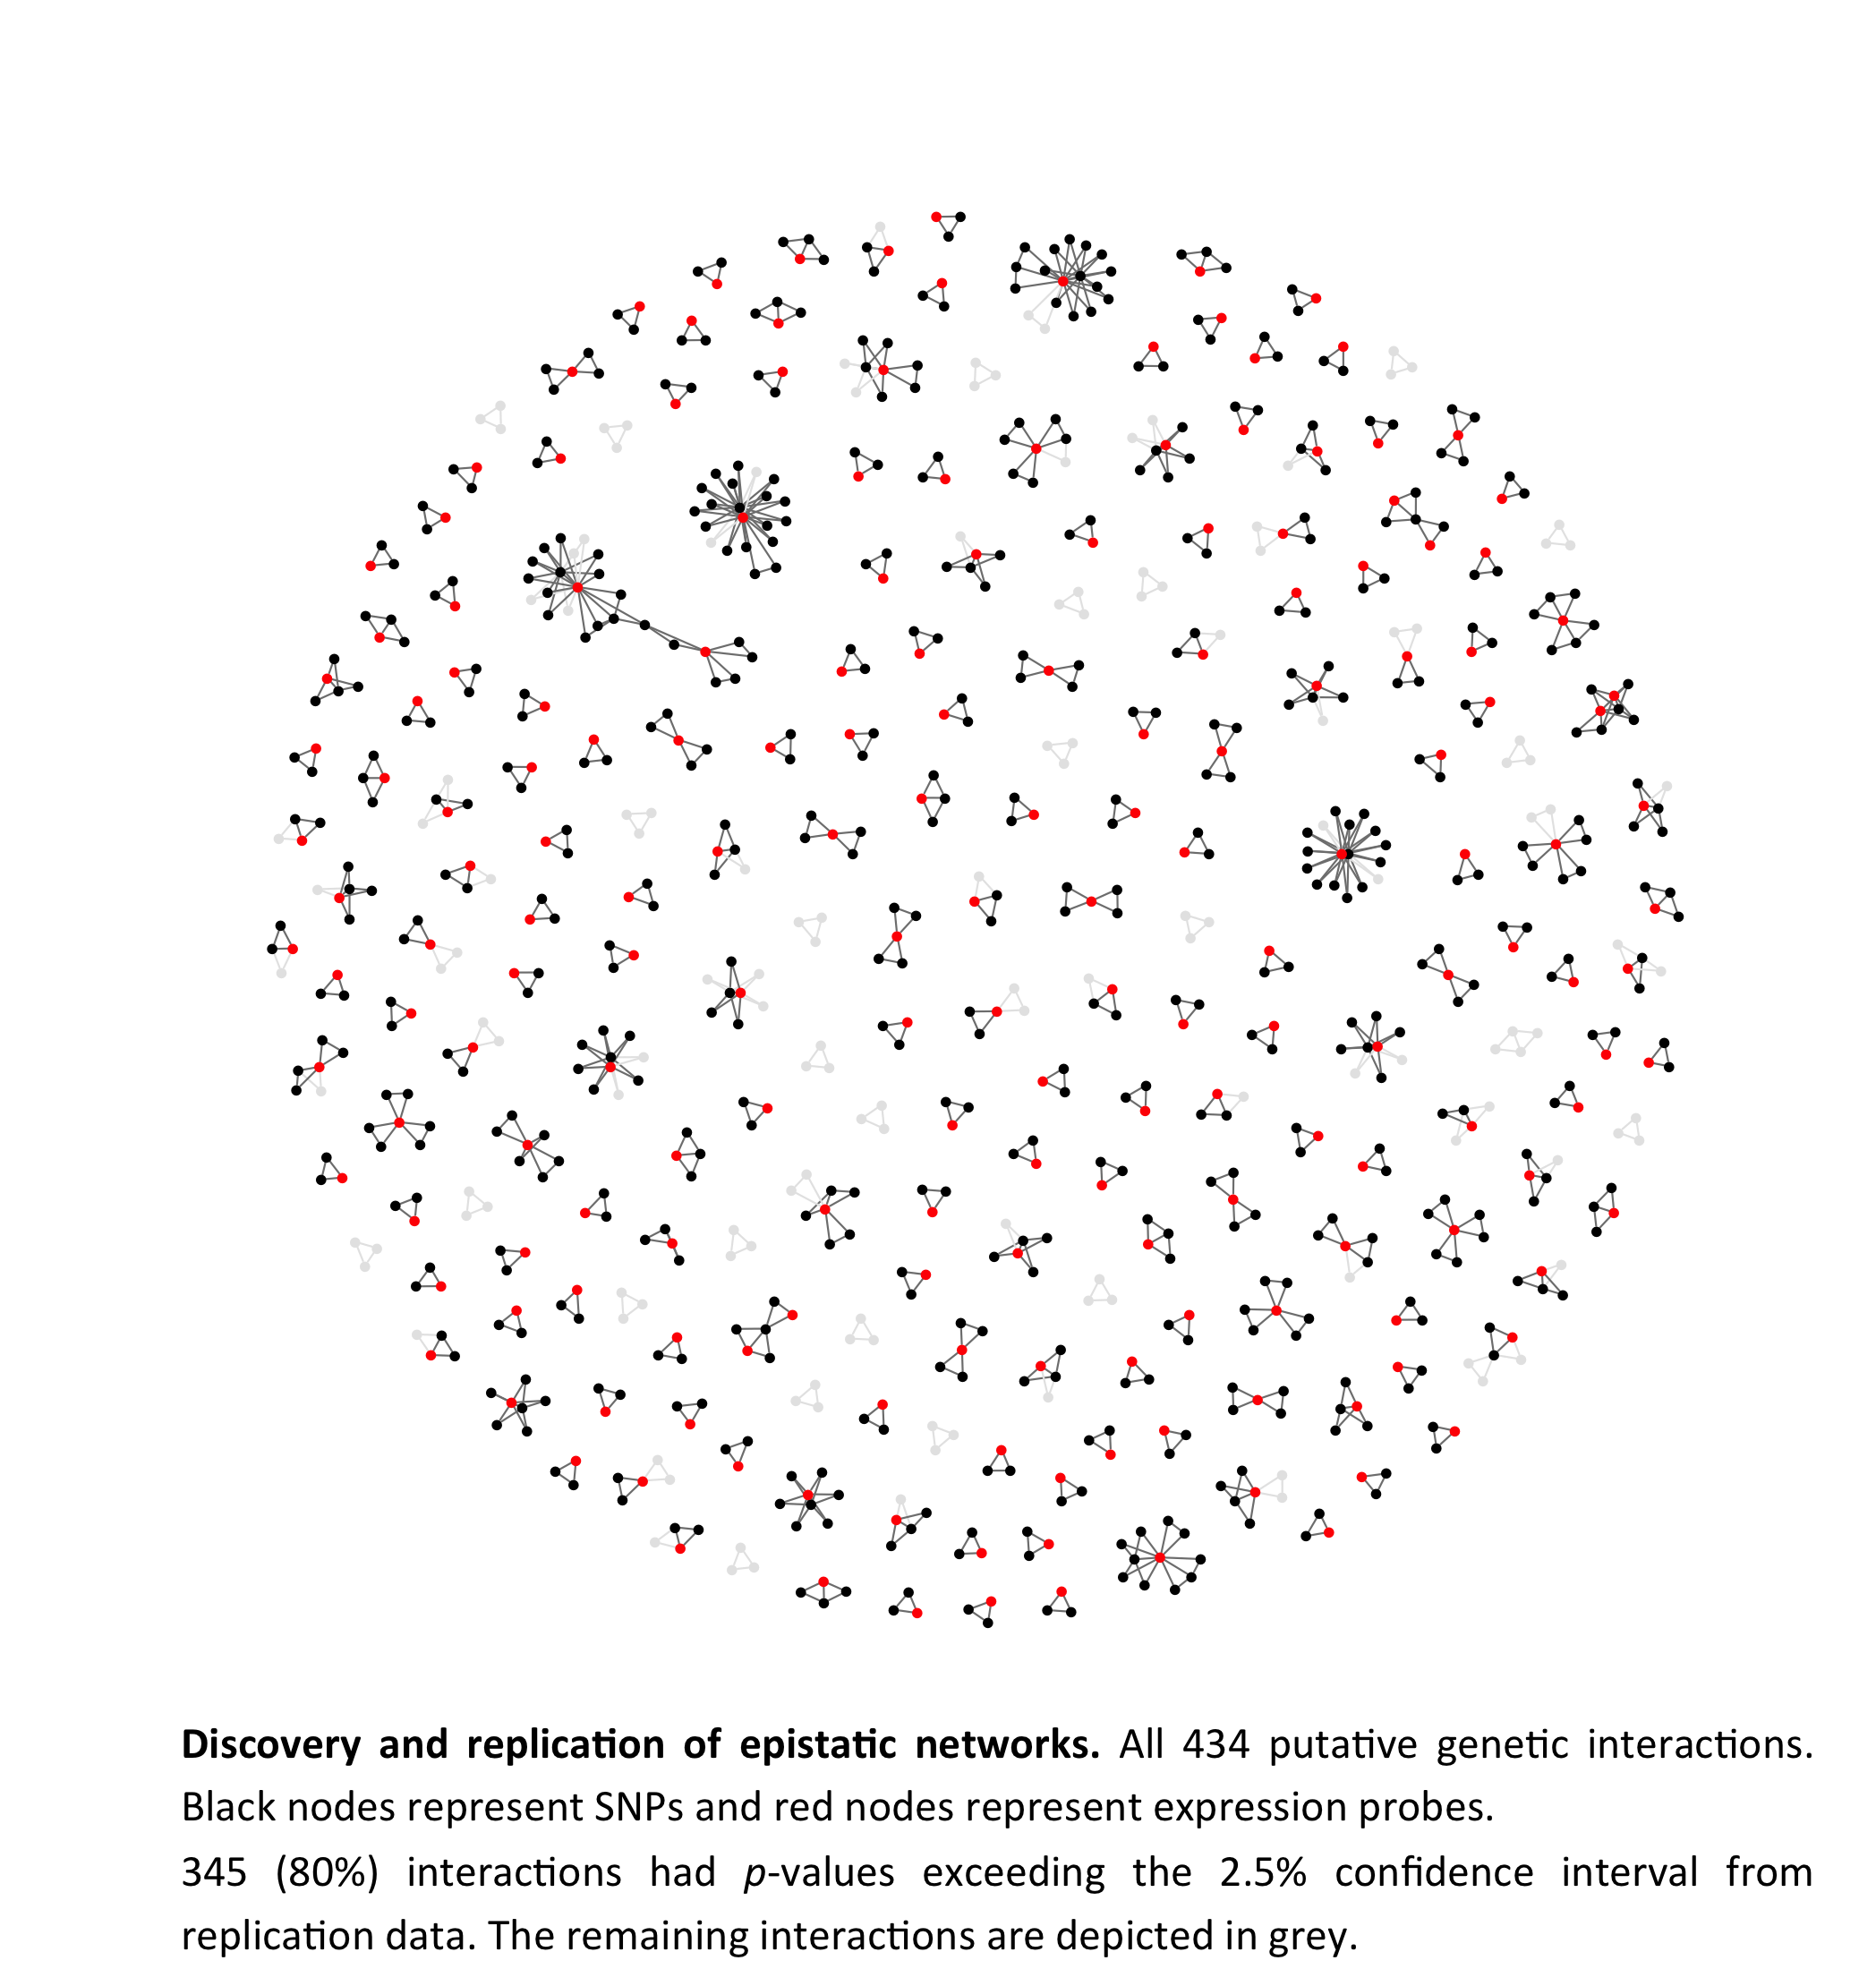
\includegraphics[height=8cm]{images/fireworks2.png} \\
\end{center}
\end{frame}

\begin{frame}{MBNL1}
\begin{columns}[c]
\column{.5\textwidth}
Involved in RNA modification and regulation of splicing \\
\vspace{0.3cm}
Has one cis-effect, controlled by 13-trans SNPs \\   
\vspace{0.3cm}
Each pair is independent \\
\vspace{0.3cm}
Masking pattern: when the trans-SNP is homozygous for the masking allele the decreasing allele of the cis-SNP no longer has an effect
\column{.5\textwidth} 
\begin{center}
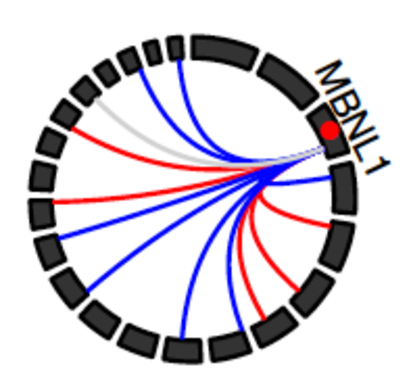
\includegraphics[height=3.0cm]{images/MBNL1.pdf} \\
\end{center}
\end{columns}
\end{frame}


\begin{frame}{Chromosome interactions}
\begin{columns}[c]
\column{.5\textwidth}
Are epistatic SNPs located in positions known to interact? 
\begin{itemize}
\item Chromosome interactions identifyed in K562 cell lines using Hi-C and ChIP-seq
\item red lines = $N$ SNPs within 20kb, 500kb, 2Mb and 10Mb of known interacting regions
\item Histograms = null distributions
\end{itemize}
\column{.5\textwidth} 
\begin{center}
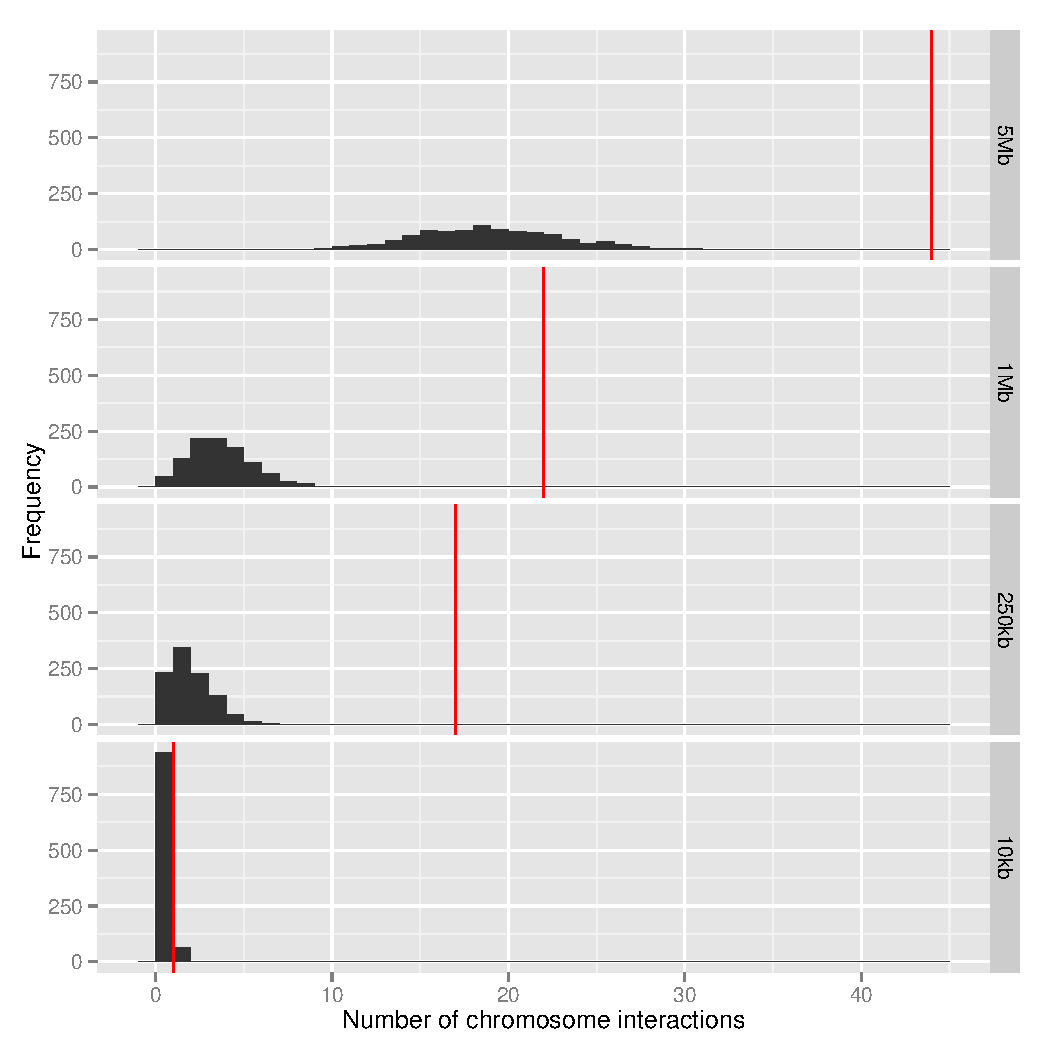
\includegraphics[height=4.5cm]{images/chr_int.pdf} \\
\end{center}
\end{columns}
\end{frame}


\begin{frame}{Conclusions}
This study presents the first evidence for multiple instances of segregating common polymorphisms interacting to influence human traits. \\
\vspace{0.4cm}
Computational and statistical frameworks can identify and replicate epistasis in complex traits. \\
\vspace{0.4cm}
Functional characterization of epistatic loci suggests a large number of possible mechanisms that can lead to non-additive genetic variation.
\end{frame}

\section*{}
\begin{frame}{Acknowledgements}
\begin{columns}
\column{.5\textwidth}
{\tiny
Complex Trait Genomics Group
\begin{itemize}
\item Gib Hemani
\item Kostya Shakhbazov
\item Jian Yang
\item Allan Mcrae
\item Peter Visscher
\end{itemize}
University of Groningen
\begin{itemize}
\item Harm-Jan Westra
\item Lude Franke
\end{itemize}
}
\column{.5\textwidth}
{\tiny
QIMR Berghofer
\begin{itemize}
\item Nick Martin
\item Anjali Henders
\item Grant Montgomery
\end{itemize}
Georgia Institute of Technology
\begin{itemize}
\item Greg Gibson
\end{itemize}
University of Tartu
\begin{itemize}
\item Andres Metspalu
\item Tonu Esko
\end{itemize}
Visit us at www.complextraitgenomics.com
}
\end{columns}
\end{frame}




\end{document}


